\chapter{Implementation, Evaluation, and Discussion}
\label{ch:pfe-evaluation}

\section{Introduction}

The architecture presented in Chapter~\ref{ch:pfe-design} was implemented as
a Python command-line system that accepts compiled Android APKs, extracts
static evidence, compares it with versioned Maven reference profiles, emits a
\CycloneDX SBOM, and optionally queries vulnerabilities. This chapter has
three objectives. First, it explains the principal implementation modules and
their failure behavior. Second, it defines an evaluation protocol that keeps
controlled, real, source-known, experimental, and limitation evidence
separate. Third, it reports both successful and failed experiments so that the
final conclusions reflect the system's actual evidence boundaries.

All numerical results in this chapter were frozen on 20 June 2026 from
generated JSON artifacts and regenerated thesis tables. The frozen snapshot is
maintained with the project evidence package and records the numerator,
denominator, evidence class, permitted interpretation, and principal
limitation of each result.

\section{Development Environment}

The implementation uses a small set of technologies selected for
reproducibility rather than for visual demonstration. Table~\ref{tab:pfe-dev-env}
summarizes their role.

\begin{table}[H]
\centering
\caption{Development and execution environment of the implemented MVP.}
\label{tab:pfe-dev-env}
\begin{tabularx}{\textwidth}{L{0.24\textwidth}L{0.21\textwidth}X}
\toprule
\textbf{Technology} & \textbf{Project version or role} & \textbf{Use}\\
\midrule
Python & 3.12 or newer & CLI orchestration, evidence extraction, matching,
validation, report generation, and evaluation scripts.\\
Androguard & 4.1.3 & Parsing DEX bytecode and recovering classes, methods,
instructions, literals, and references.\\
NetworkX & 3.4.2 & Graph-oriented dependency representations and structural
diagnostics.\\
SQLite & Embedded database & Persistent coordinate/version profiles and child
feature tables.\\
Android build tools & D8, build-tools 36.0.0 & Conversion of JAR/AAR bytecode
into the same DEX representation analyzed in APKs.\\
Docker and Compose & Containerized toolchain & Android SDK, Java, Gradle
compatibility versions, scanners, and isolated project execution.\\
\CycloneDX & Specification 1.5 & Standard JSON SBOM representation
\cite{cyclonedxSpecification}.\\
OSV & Maven package/version lookup & Ecosystem-aware vulnerability queries for
accepted Maven detections.\\
Pytest & Development verification & Unit and integration-oriented regression
tests.\\
\bottomrule
\end{tabularx}
\end{table}

The Docker image includes Java, Android command-line tools, D8, several Gradle
versions, and optional external SBOM scanners. Multiple Gradle versions are
necessary because the real-APK source-validation set contains both modern and
legacy Android projects. The core matcher itself does not require network
access after the APK and SQLite reference database are available. Network
access is needed only for operations such as Maven acquisition and OSV
queries.

During the final evidence freeze, the local project virtual environment passed
all 275 tests in 34.64 seconds. A separate compilation check over
\path{src/}, \path{scripts/}, and \path{tests/} also passed. These checks verify
the current Python implementation; they do not replace APK-level target and
control evaluations.

\section{Implementation by Module}

\subsection{Module Map}

Table~\ref{tab:pfe-module-map} maps the implemented responsibilities to their
principal source files. The implementation deliberately separates extraction,
matching, SBOM generation, vulnerability interpretation, and source
validation so that a failure in one stage does not silently become evidence
for another.

\begin{table}[H]
\centering
\caption{Principal implementation modules and their observable outputs.}
\label{tab:pfe-module-map}
\begin{tabularx}{\textwidth}{L{0.21\textwidth}L{0.30\textwidth}X}
\toprule
\textbf{Module} & \textbf{Principal source} & \textbf{Responsibility and output}\\
\midrule
CLI & \path{src/apk_sbom/cli.py} & Parses commands and flags, selects stable or
experimental paths, and writes structured command output.\\
APK extractor & \path{src/apk_sbom/apk_extractor.py} & Validates the APK
archive; records hashes, manifest data, DEX entries, native files, and
forensic indicators.\\
DEX analyzer & \path{src/apk_sbom/dex_analyzer.py} & Aggregates package,
class, method, opcode, literal, API, and dependency evidence across all
recoverable DEX files.\\
Reference acquisition & \path{src/apk_sbom/maven_downloader.py} & Downloads
versioned JAR/AAR artifacts, POM metadata, declared dependencies, and
checksums.\\
Reference conversion & \path{src/apk_sbom/reference_converter.py} & Extracts
AAR bytecode when required and invokes D8 to obtain comparable DEX files.\\
Feature database & \path{src/apk_sbom/reference_features.py} & Transactionally
stores one component row per coordinate/version and its child feature rows.\\
Matcher & \path{src/apk_sbom/matcher.py} & Scores candidate profiles,
separates identity from version confidence, records alternatives, and applies
guarded family logic.\\
SBOM generator & \path{src/apk_sbom/sbom.py} & Produces \CycloneDX 1.5
components, Package URLs, evidence properties, and native file hashes.\\
Vulnerability layer & \path{src/apk_sbom/vulnerability.py} & Queries OSV,
deduplicates aliases, extracts severity, and applies certainty labels.\\
Report generator & \path{src/apk_sbom/report.py} & Orchestrates the full
pipeline and writes JSON, Markdown, and HTML reports.\\
Source validator & \path{src/apk_sbom/source_validation.py} & Compares emitted
Maven components with resolved Gradle dependency evidence.\\
AI/R8 assistants & \path{src/apk_sbom/ai_r8_assistant.py} and related modules &
Produce report-only risk and investigation suggestions without changing
authoritative output.\\
\bottomrule
\end{tabularx}
\end{table}

\subsection{Extraction and DEX Analysis}

The extractor first checks that the input is a readable ZIP/APK archive and
computes its SHA-256 hash. It discovers both standard
\path{classes*.dex} entries and DEX files in unusual paths. The latter are
retained as forensic indicators because hidden or dynamically loaded code
cannot be treated as ordinary statically recovered application logic.

Manifest metadata includes the package name, version name, version code,
minimum SDK, target SDK, and declared permissions. Native
\path{.so} entries are recorded with their ABI, path, size, and hash. They are
not converted into Maven identities because the current reference pipeline is
designed for JVM/Android bytecode artifacts.

The DEX analyzer parses each discovered DEX independently and then aggregates
the successfully recovered evidence. A parse error is retained in the output;
it is not converted into an empty-feature result. The default score uses
packages, class descriptors, method signatures, opcode histograms, class
dependencies, dependency-shape summaries, literals, and version-unique
class/method/literal evidence. API-reference and opcode n-gram features are
extracted but have zero default weight. The guarded version-unique
literal/context reranker and composite family shortlist are enabled by
default, while broader basic-block, call-chain, class-neighbor,
field-operation, and multi-scale features remain diagnostic or report-only.

\subsection{Reference Construction}

The reference pipeline begins with a catalog of Maven coordinates and selected
versions. Each artifact is downloaded with provenance metadata and a SHA-256
hash. JAR artifacts are passed directly to D8. For AAR artifacts, the
converter extracts \path{classes.jar} first. Resource-only, POM-only, and
source-wrapper artifacts are recorded as no-bytecode outcomes instead of
being represented as empty libraries.

Converted references are processed by the same DEX analyzer used for APKs.
This shared representation reduces a major comparison mismatch: APK evidence
is compared with compiled reference evidence rather than source-code
descriptions. The SQLite database stores one unique component row for each
coordinate/version pair and child rows for every feature family. Re-extraction
clears and rewrites the selected component's child rows transactionally.

Exploratory growth never writes directly into the shared calibrated database.
Focused, priority, large, and single-coordinate experiments use separate
SQLite paths. A reference addition becomes eligible for shared promotion only
after target improvements and current controls are evaluated.

\subsection{Evidence Scoring and Version Decisions}

For a candidate component \(c\), the matcher combines the configured feature
scores using a normalized weighted sum:

\begin{equation}
S(c)=\frac{\sum_{i \in F} w_i s_i(c)}
{\sum_{i \in F} w_i},
\label{eq:pfe-matcher-score}
\end{equation}

where \(F\) is the configured feature set, \(s_i(c)\) is the corresponding
similarity or coverage score, and \(w_i\) is its configured weight. A missing
or empty reference feature family contributes a score of zero; a disabled
family has weight zero. The default weights are shown in
Table~\ref{tab:pfe-matcher-weights}. The resulting value is a ranking score,
not a calibrated probability.

\begin{table}[H]
\centering
\caption{Default matcher weights in the authoritative path.}
\label{tab:pfe-matcher-weights}
\begin{tabular}{lr@{\hspace{14mm}}lr}
\toprule
\textbf{Feature} & \textbf{Weight} & \textbf{Feature} & \textbf{Weight}\\
\midrule
Package coverage & 0.15 & Class coverage & 0.45\\
Method coverage & 0.25 & Opcode similarity & 0.15\\
Dependency similarity & 0.10 & Literal overlap & 0.08\\
Version-unique evidence & 0.12 & API references & 0.00\\
Opcode tri-grams & 0.00 & &\\
\bottomrule
\end{tabular}
\end{table}

Only features with nonzero configured weights contribute to the normalized
denominator. The zero default values are intentional: API-reference and opcode
tri-gram experiments did not justify global production weight. The class
signal receives the largest weight because it is discriminative in clear
cases, while structural, opcode, and literal evidence reduce dependence on
preserved names.

Candidate versions are grouped by coordinate. The matcher records the best
candidate, score gap, alternatives, ambiguity reason, and any versions close
enough to form an ambiguous set. Identity confidence answers whether the
library family is supported; version confidence answers whether one release
is sufficiently separated from sibling versions. A strong identity can
therefore coexist with an uncertain exact version.

\subsection{SBOM, Vulnerability, and Reporting Layers}

Accepted Maven decisions become \CycloneDX components with group, artifact,
version, PURL, confidence labels, match type, ambiguity properties, and
evidence summaries. Native files become \CycloneDX file components with hashes
and metadata. Uncertain Maven decisions are excluded by default; an explicit
flag is required to include them.

The vulnerability layer sends Maven coordinate/version pairs to the OSV batch
endpoint. Returned OSV, GHSA, and CVE identifiers are deduplicated, and
severity data is extracted when available. A source-validation artifact can
then relabel a finding as source-confirmed, source-version-mismatch,
source-missing, or report-only. This policy prevents a correct vulnerability
lookup on an incorrect selected version from being presented as a confirmed
application vulnerability.

The report generator writes:

\begin{itemize}
  \item \path{matches.json}, containing ranked candidates and decisions;
  \item \path{sbom.cdx.json}, containing the standard SBOM;
  \item \path{osv-vulnerabilities.json}, when OSV is enabled;
  \item \path{report.json}, the combined machine-readable evidence;
  \item \path{report.md} and \path{report.html}, the human-readable reports.
\end{itemize}

Optional AI, R8, version-band, and hybrid sections are loaded as attachments.
They can add explanatory text but cannot modify selected versions, SBOM
components, vulnerability labels, or source-validation metrics.

\section{Command-Line Workflow}

\subsection{Minimal APK-to-Report Run}

The ordinary workflow requires an APK and an existing SQLite reference
database:

\begin{lstlisting}[style=thesiscode,
caption={Minimal deterministic end-to-end report command.}]
docker compose run --rm apk-sbom python -m apk_sbom.cli generate-report \
  path/to/application.apk \
  --db-path data/reference_db/reference_features_calibrated_combined.sqlite \
  --output-dir data/results/application-report
\end{lstlisting}

For an offline or deterministic matcher run, \path{--skip-osv} disables
network queries without changing extraction, matching, SBOM generation, or
report creation. The \path{--include-uncertain} flag changes the meaning of the
SBOM because uncertain decisions become components; it should therefore be
used only for diagnostic consumers.

\subsection{Diagnostic Commands}

The system exposes narrower commands for inspecting individual stages:

\begin{table}[H]
\centering
\caption{Core CLI commands and their expected result.}
\label{tab:pfe-core-commands}
\begin{tabularx}{\textwidth}{L{0.29\textwidth}X}
\toprule
\textbf{Command} & \textbf{Expected result}\\
\midrule
\path{inspect-apk APK} & Archive, manifest, DEX, native-file, hash, and
forensic evidence; no component matching.\\
\path{analyze-dex APK} & Aggregated bytecode feature counts and parse errors.\\
\path{match-apk APK} & Ranked reference candidates and separate
identity/version decisions.\\
\path{generate-sbom APK} & \CycloneDX JSON built from accepted matcher
decisions.\\
\path{scan-sbom-osv SBOM} & OSV vulnerability JSON for Maven components.\\
\path{generate-report APK} & Complete evidence package in JSON, Markdown, and
HTML.\\
\path{validate-source-deps} & Confirmed, version-mismatch, and missing
classifications against a Gradle dependency tree.\\
\bottomrule
\end{tabularx}
\end{table}

The \path{--coordinate group:artifact} flag is valuable for diagnosis, but it
supplies the library identity externally. Results obtained with that flag are
coordinate-constrained separability tests, not ordinary unconstrained APK
detection.

\subsection{Reference-Database Workflow}

A reproducible reference build follows four commands:

\begin{lstlisting}[style=thesiscode,
caption={Reference-database construction workflow.}]
apk-sbom expand-reference-config \
  --catalog configs/popular_android_maven_catalog.json \
  --output configs/libraries.reproduction.json --latest-count 1 --limit 5
apk-sbom download-maven --config configs/libraries.reproduction.json \
  --output-root data/reference_db/artifacts_reproduction
apk-sbom convert-reference-dex \
  --artifact-root data/reference_db/artifacts_reproduction \
  --output-root data/reference_db/dex_reproduction
apk-sbom extract-reference-features \
  --dex-root data/reference_db/dex_reproduction \
  --db-path data/reference_db/reference_features_reproduction.sqlite
\end{lstlisting}

The destructive \path{--reset} flag is used only when creating an explicitly
rebuildable database. Later batches append or replace individual
coordinate/version rows. Experimental paths must remain distinct from the
shared calibrated database.

\section{Evaluation Methodology}

\subsection{Research Questions}

The evaluation operationalizes the four research questions introduced in
Chapter~\ref{ch:pfe-introduction}:

\begin{enumerate}[label=\textbf{RQ\arabic*:}]
  \item Can the pipeline recover exact Maven versions when ground truth and
  adequate reference evidence are available?
  \item How does emitted-version quality change between clean and difficult
  real APK families?
  \item How much of the full source dependency denominator is represented by
  the reference database and emitted by the matcher?
  \item Can SBOM, vulnerability, and AI assistance preserve uncertainty and
  authority boundaries?
\end{enumerate}

\subsection{Evidence Layers}

The datasets are not merged into one accuracy number. Their roles are defined
in Table~\ref{tab:pfe-evidence-layers}.

\begin{table}[H]
\centering
\caption{Evaluation layers and permitted claims.}
\label{tab:pfe-evidence-layers}
\begin{tabularx}{\textwidth}{L{0.23\textwidth}L{0.15\textwidth}X}
\toprule
\textbf{Layer} & \textbf{Cases} & \textbf{Ground truth and permitted use}\\
\midrule
Controlled fixtures & 72 & Exact by construction; used for expected component
and version confirmation across clear, R8, repackaging, multidex, and
multi-library categories.\\
Clean source-validated real APKs & 5 & Resolved source dependency trees and no
emitted mismatch; strongest real emitted-version evidence.\\
Partial source-validated real APKs & 97 & Resolved source evidence with
explicit mismatches or nuanced rows; used to characterize difficult families.\\
Source-validated no-Maven-signal controls & 4 & Resolved runtime dependency
trees, but zero emitted Maven components; excluded from the emitted-version
rate and retained as matcher-recall and emission-threshold controls.\\
Source-known v2 lane & 106 & Exact source coordinate/version slices; used only
as a recognition and reference-coverage upper bound.\\
Limitation cases & 4 & Native-heavy, hidden-code, or obfuscated samples; used
to evaluate warnings and scope, not Maven-version accuracy.\\
Report-only and experiment-only lanes & varies & Used to evaluate potential
improvements without changing authoritative output.\\
\bottomrule
\end{tabularx}
\end{table}

\subsection{Metrics and Denominators}

For controlled fixtures, exact expected-version confirmation is:

\begin{equation}
R_{\mathrm{controlled}} =
\frac{\text{expected coordinate/version pairs recovered exactly}}
{\text{expected coordinate/version pairs}}.
\end{equation}

For source-validated real APKs, emitted Maven version confirmation is:

\begin{equation}
C_{\mathrm{emitted}} =
\frac{\text{emitted Maven rows confirmed by source}}
{\text{emitted Maven rows checked against source}}.
\label{eq:pfe-emitted-confirmation}
\end{equation}

Equation~\ref{eq:pfe-emitted-confirmation} measures the quality of emitted
rows. It is not full dependency recall. The full-denominator exact source
recall is:

\begin{equation}
R_{\mathrm{source}} =
\frac{\text{source dependency rows emitted with exact version}}
{\text{resolved source dependency coordinate/version rows}}.
\label{eq:pfe-source-recall}
\end{equation}

The evaluation also records version mismatches and missing or nuanced rows.
The latter category includes emitted coordinates absent from the supplied
source tree and artifact-family situations requiring separate interpretation.

\subsection{Regression and Promotion Protocol}

Every scoring, reference, shortlist, or reranking proposal follows a fail-fast
protocol:

\begin{enumerate}
  \item create an isolated implementation or SQLite database;
  \item run one or more intended target cases;
  \item run controlled, clean, partial, no-Maven, and boundary controls
  appropriate to the proposal;
  \item stop when a material regression already blocks safe promotion;
  \item classify the outcome as promoted, report-only, experiment-only,
  rejected, or blocked.
\end{enumerate}

A target improvement alone is insufficient. This rule is especially important
for adjacent AndroidX and Kotlin versions, where tiny score differences may
reverse between applications.

\section{Controlled Evaluation}

The controlled inventory contains 72 APK fixtures and 84 expected Maven
coordinate/version pairs. It covers clear version bands, R8 rename, R8 shrink,
R8 optimization, shrink plus optimization, package flattening, inline-like
call-site stress, multidex packaging, and multi-library combinations.

\begin{table}[H]
\centering
\caption{Controlled evaluation by transformation category.}
\label{tab:pfe-controlled-categories}
\begin{tabularx}{\textwidth}{Xrr}
\toprule
\textbf{Controlled category} & \textbf{Cases} & \textbf{Exact expected versions}\\
\midrule
Clear fixtures & 25 & 25/25\\
R8 rename & 8 & 8/8\\
R8 shrink & 8 & 8/8\\
R8 optimize & 6 & 6/6\\
R8 shrink and optimize & 6 & 6/6\\
Package flattening/repackaging & 6 & 6/6\\
Inline-like call-site stress & 6 & 6/6\\
Multidex and multi-library & 7 & 19/19\\
\midrule
\textbf{Total} & \textbf{72} & \textbf{84/84}\\
\bottomrule
\end{tabularx}
\end{table}

The 84/84 result establishes that the implemented pipeline can recover the
expected versions across the controlled inventory. It does not establish
perfect real-world behavior. Controlled fixtures contain known artifacts,
known transformations, and reference coverage selected by construction.
Their principal role is to guard mechanics and detect regressions.

\section{Source-Validated Real-APK Evaluation}

\subsection{Main Emitted-Version Results}

Table~\ref{tab:pfe-main-real-results} reports clean and partial APKs separately
before presenting the aggregate.

\begin{table}[H]
\centering
\caption{Source-validated emitted Maven version results.}
\label{tab:pfe-main-real-results}
\begin{tabularx}{\textwidth}{Xrrrrrr}
\toprule
\textbf{Slice} & \textbf{Cases} & \textbf{Checked} & \textbf{Exact} &
\textbf{Wrong} & \textbf{Missing/nuance} & \textbf{Rate}\\
\midrule
Clean real APKs & 5 & 47 & 47 & 0 & 0 & 100.0\%\\
Partial real APKs & 97 & 1,790 & 880 & 636 & 274 & 49.2\%\\
\midrule
\textbf{Source-validated APKs with emitted Maven rows} & \textbf{102} &
\textbf{1,837} &
\textbf{927} & \textbf{636} & \textbf{274} & \textbf{50.5\%}\\
\bottomrule
\end{tabularx}
\end{table}

The clean set contains F-Droid, OpenTracks, Tusky, Daily Dozen, and QuickDic.
F-Droid and OpenTracks provide richer component sets. Tusky, Daily Dozen, and
QuickDic are clean but sparse, with only one or two emitted Maven components.
Consequently, the 47/47 result is strong evidence for those emitted rows but
cannot represent every real APK family.

The partial set contains modern AndroidX/Kotlin applications, minified and R8
cases, email and security applications, native-heavy frameworks, older
dependency eras, and large dependency trees. Confirming 880 of 1,790 emitted
versions shows that the output remains useful, while the 636 wrong-version and
274 missing/nuanced rows expose the cost of nearby version similarity,
artifact-family differences, and incomplete reference coverage.

Across the 102 source-validated APKs that emitted Maven components, 927 of
1,837 emitted versions are confirmed exactly. The resulting 50.5\% is
therefore called the \emph{emitted Maven version confirmation rate}. It must
not be described as full dependency recall.

Four additional source-validated cases---Privacy Browser, Mastodon, monocles
browser, and Blue Square Speedometer---have resolved runtime dependency trees
but emit zero Maven components. They are excluded from the 927/1,837 metric
because they provide no emitted rows to score; they remain separate
matcher-recall and emission-threshold controls and are included in the full
106-case source denominator.

\subsection{Full Source Dependency Denominator}

The resolved source trees contain 12,082 coordinate/version rows across 106
source-tree cases. The distinction between emission quality and coverage is
shown in Table~\ref{tab:pfe-coverage-first}.

\begin{table}[H]
\centering
\caption{Coverage-first view of the full source dependency denominator.}
\label{tab:pfe-coverage-first}
\begin{tabularx}{\textwidth}{Xrr}
\toprule
\textbf{Metric} & \textbf{Rows} & \textbf{Rate}\\
\midrule
Source rows whose coordinate exists in the shared DB & 2,220/12,082 & 18.4\%\\
Source rows whose exact coordinate/version exists in the shared DB &
1,231/12,082 & 10.2\%\\
Source rows emitted with the exact source version & 927/12,082 & 7.7\%\\
\bottomrule
\end{tabularx}
\end{table}

This result changes the interpretation of the 50.5\% metric. Among rows the
system emitted, approximately half of the versions are source-confirmed.
Against the full source dependency denominator, only 7.7\% are emitted
exactly. Some source rows are metadata-only, platform, alias, transformed, or
removed before packaging, but the denominator still reveals that both
reference coverage and matcher recall remain major limitations.

\section{Source-Known Upper-Bound Evaluation}

The final v2 evaluation addresses a narrower question: if the exact
source-observed coordinate/version profiles are known and the search space is
restricted to those profiles, can the system recognize and report them
without emitting wrong versions?

The v2 database contains 10,517 component profiles. For each source-tree APK,
the evaluator constructed a slice containing exact coordinate/version rows
from its resolved source dependency tree. All 106 cases completed.

\begin{table}[H]
\centering
\caption{Source-version constrained v2 upper-bound results.}
\label{tab:pfe-v2-results}
\begin{tabularx}{\textwidth}{Xr}
\toprule
\textbf{Metric} & \textbf{Value}\\
\midrule
Completed source-tree cases & 106/106\\
Emitted rows checked & 6,772\\
Exact source confirmations & 6,772\\
Wrong-version emitted rows & 0\\
Missing emitted rows & 0\\
Remaining source-gap rows & 5,238\\
\bottomrule
\end{tabularx}
\end{table}

The 6,772/6,772 result is a source-version constrained recognition upper bound,
not unconstrained APK-only production accuracy. Source knowledge changes the
candidate space and removes the ordinary version-selection problem.

The remaining 5,238 source-gap rows were not hidden. Their principal
actionable groups are 2,281 matcher-recall candidates, where an exact
reference exists but the system did not emit it, and 442 missing-reference
candidates. The other
rows include metadata/source-only artifacts, target-artifact aliases, project
modules, platform/common-source boundaries, relocated coordinates, and
already-covered siblings. This taxonomy shows that adding versions alone
cannot solve every missing source row.

\section{Vulnerability Demonstration}

Three evidence levels are used for vulnerability reporting:

\begin{enumerate}
  \item an exact controlled component/version can support a confirmed
  demonstration;
  \item a source-confirmed real emitted component/version can support a
  source-validated finding;
  \item a version mismatch, ambiguous selection, or unvalidated row remains
  potential or report-only.
\end{enumerate}

\begin{table}[H]
\centering
\caption{Representative vulnerability demonstrations and their authority.}
\label{tab:pfe-vulnerability-demo}
\begin{tabularx}{\textwidth}{L{0.28\textwidth}L{0.26\textwidth}X}
\toprule
\textbf{Case} & \textbf{Observed result} & \textbf{Interpretation}\\
\midrule
Calibrated F-Droid & 23/23 emitted Maven versions source-confirmed; 0 OSV
vulnerabilities & Clean negative demonstration.\\
Controlled Jackson Databind & Exact
\path{jackson-databind@2.9.10.8}; three HIGH advisories:
CVE-2020-36518, CVE-2022-42003, and CVE-2022-42004 &
Controlled positive demonstration.\\
Real-APK OSV triage & Eight advisories across six component rows: one
source-confirmed, six source-version-mismatch, and one report-only &
Only the source-confirmed row is source-validated vulnerability evidence.\\
\bottomrule
\end{tabularx}
\end{table}

The prototype also produces a dashboard-style HTML report that can be inspected
by an analyst. Figures~\ref{fig:pfe-dashboard-clean-summary}
to~\ref{fig:pfe-dashboard-vulnerable-tail} reproduce the complete rendered
dashboards for the clean F-Droid lane and the controlled vulnerable Jackson
lane in consecutive readable panels. These are browser captures of the actual
\path{report.html} artifacts, not manually reconstructed mock-ups. The same
runs also produced \path{report.json}, \path{report.md},
\path{sbom.cdx.json}, \path{matches.json}, and
\path{osv-vulnerabilities.json}. The figures therefore demonstrate the
implemented end-to-end output path without introducing a new evaluation
denominator.

\begin{figure}[p]
\centering
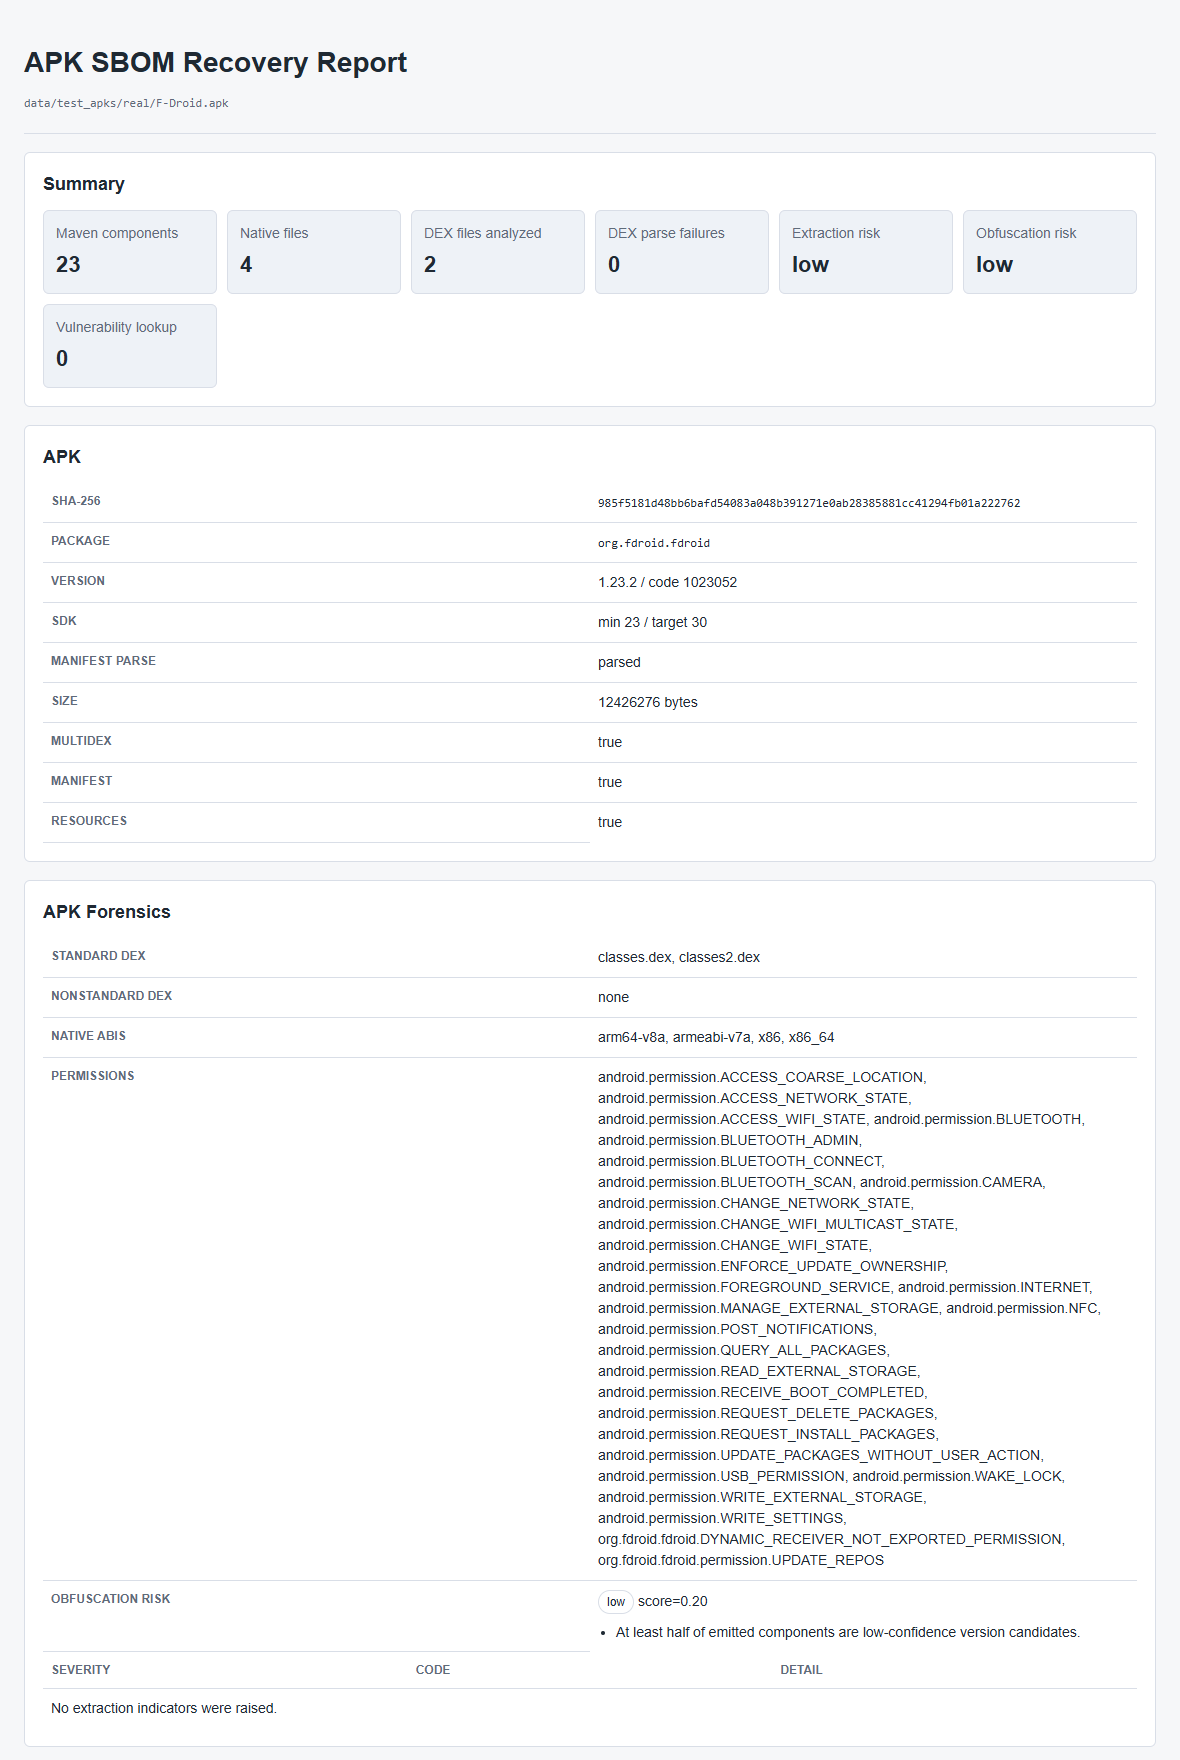
\includegraphics[width=\textwidth,height=0.78\textheight,keepaspectratio]{figures/clean-dashboard-01-summary.png}
\caption[Clean dashboard: summary and APK evidence]{Beginning of the complete
clean F-Droid HTML dashboard: report summary, APK metadata, forensic
extraction evidence, 23 detected Maven components, and zero vulnerability
findings.}
\label{fig:pfe-dashboard-clean-summary}
\end{figure}

\begin{figure}[p]
\centering
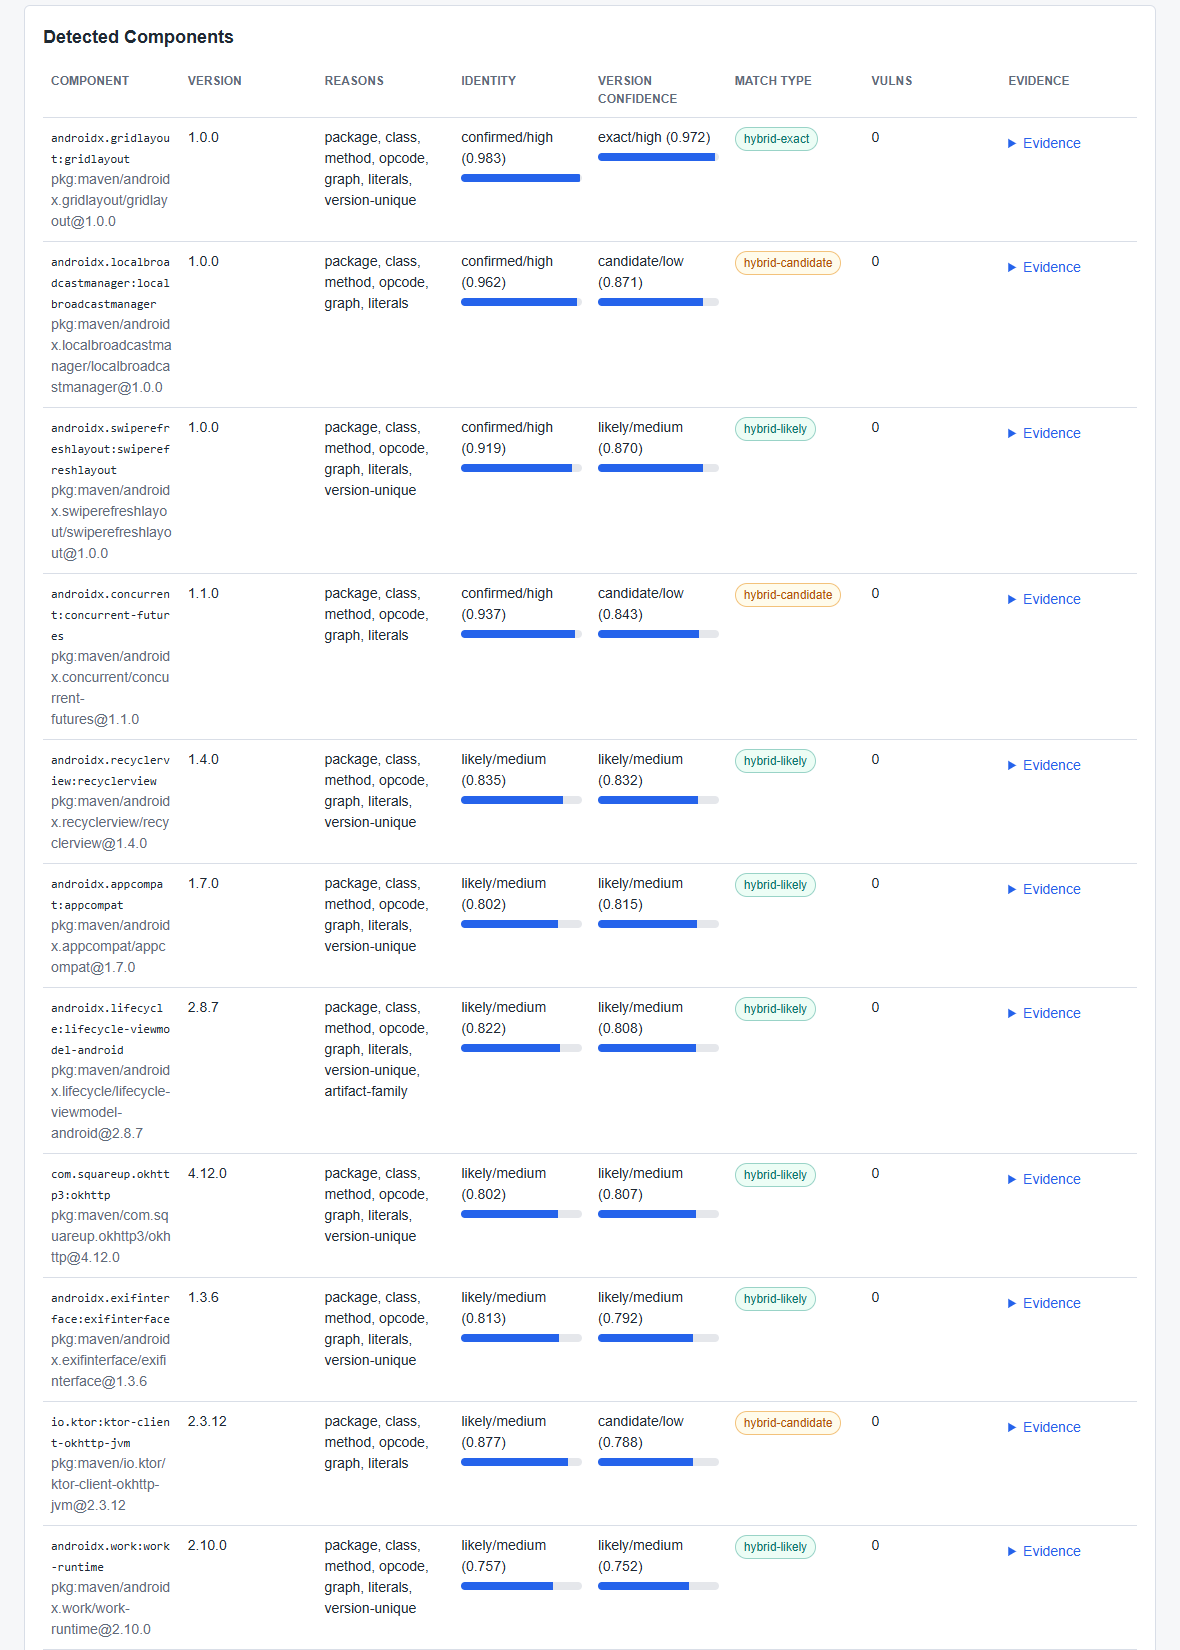
\includegraphics[width=\textwidth,height=0.78\textheight,keepaspectratio]{figures/clean-dashboard-02-components-a.png}
\caption[Clean dashboard: detected components I]{Clean F-Droid dashboard,
detected-components panel, part I. Each emitted component exposes its selected
version, evidence families, identity confidence, version confidence, match
type, vulnerability count, and expandable evidence link.}
\label{fig:pfe-dashboard-clean-components-a}
\end{figure}

\begin{figure}[p]
\centering
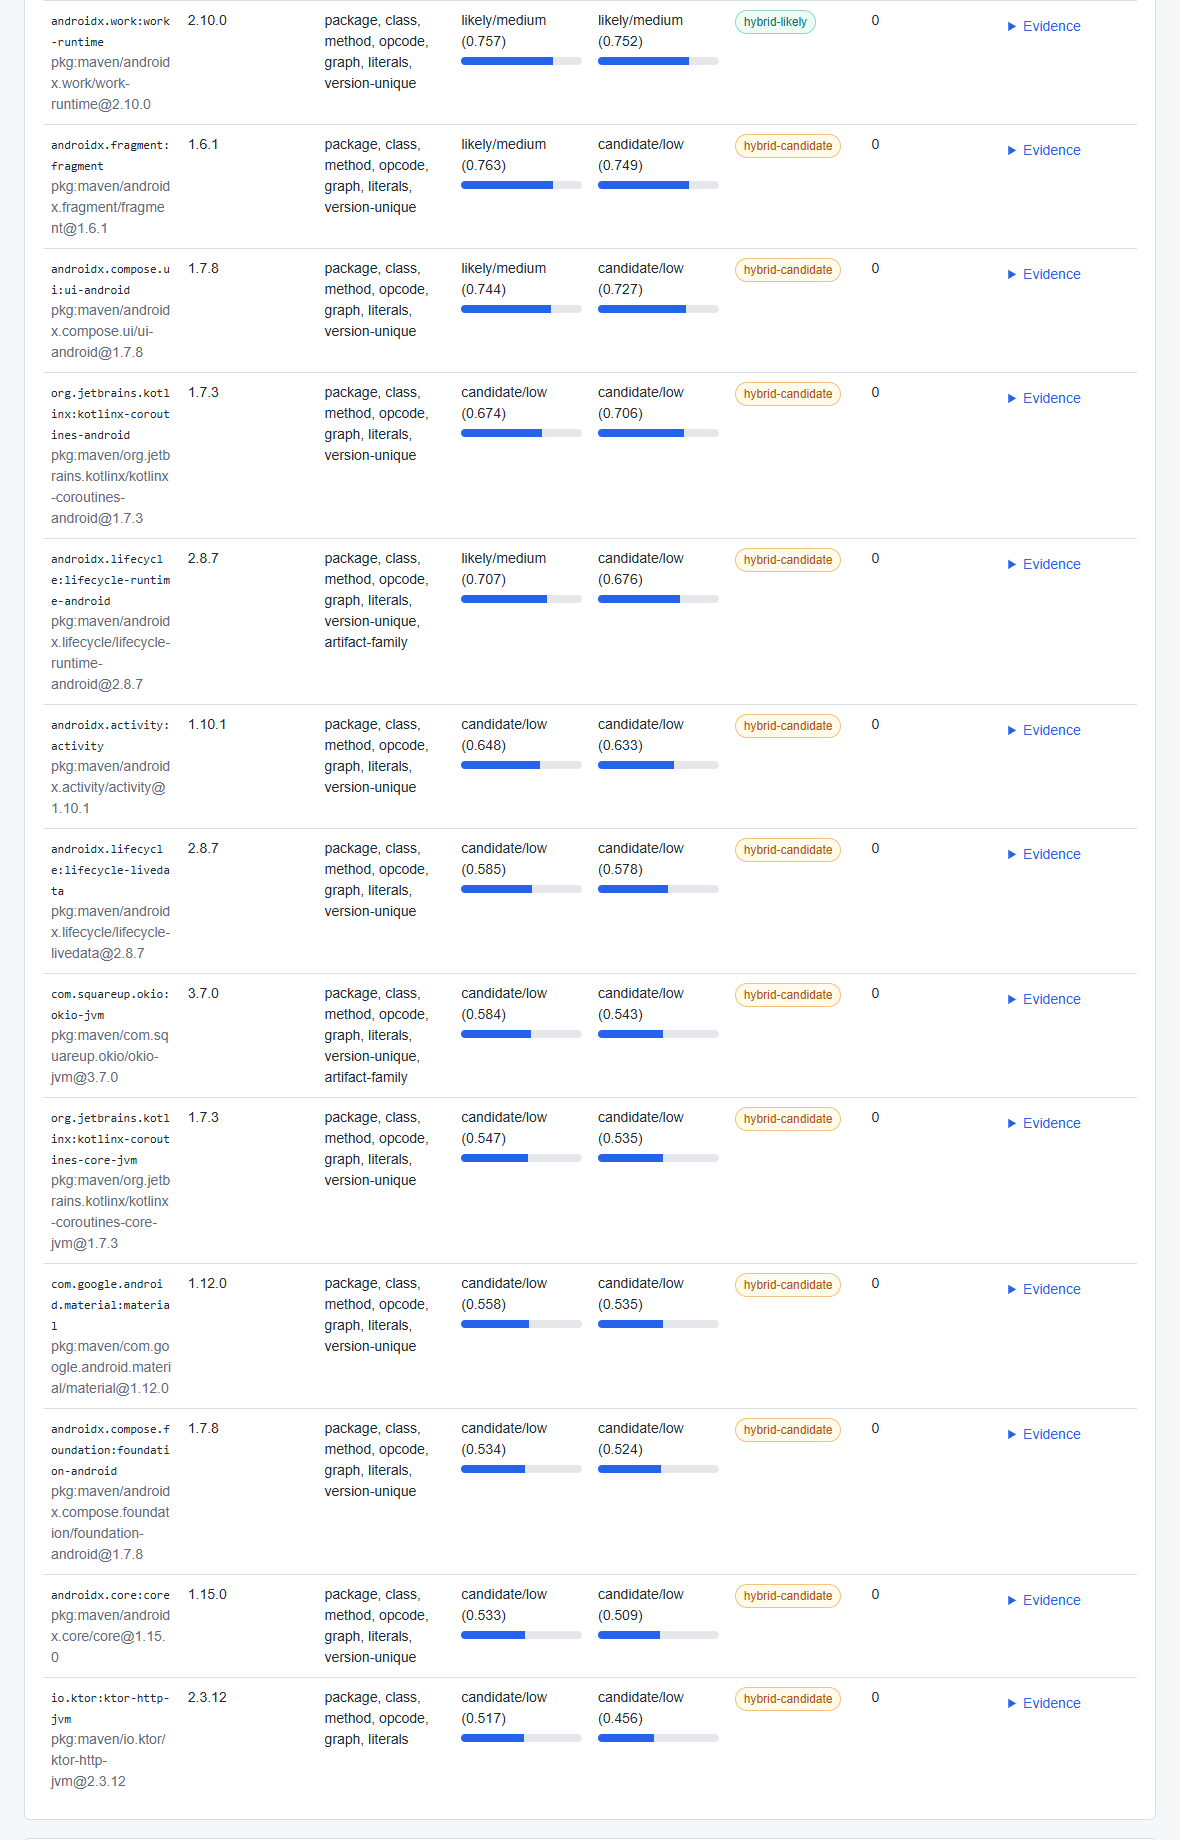
\includegraphics[width=\textwidth,height=0.78\textheight,keepaspectratio]{figures/clean-dashboard-03-components-b.png}
\caption[Clean dashboard: detected components II]{Clean F-Droid dashboard,
detected-components panel, part II. This continuation completes the component
list while preserving candidate and uncertainty labels instead of presenting
every row as an exact match.}
\label{fig:pfe-dashboard-clean-components-b}
\end{figure}

\begin{figure}[p]
\centering
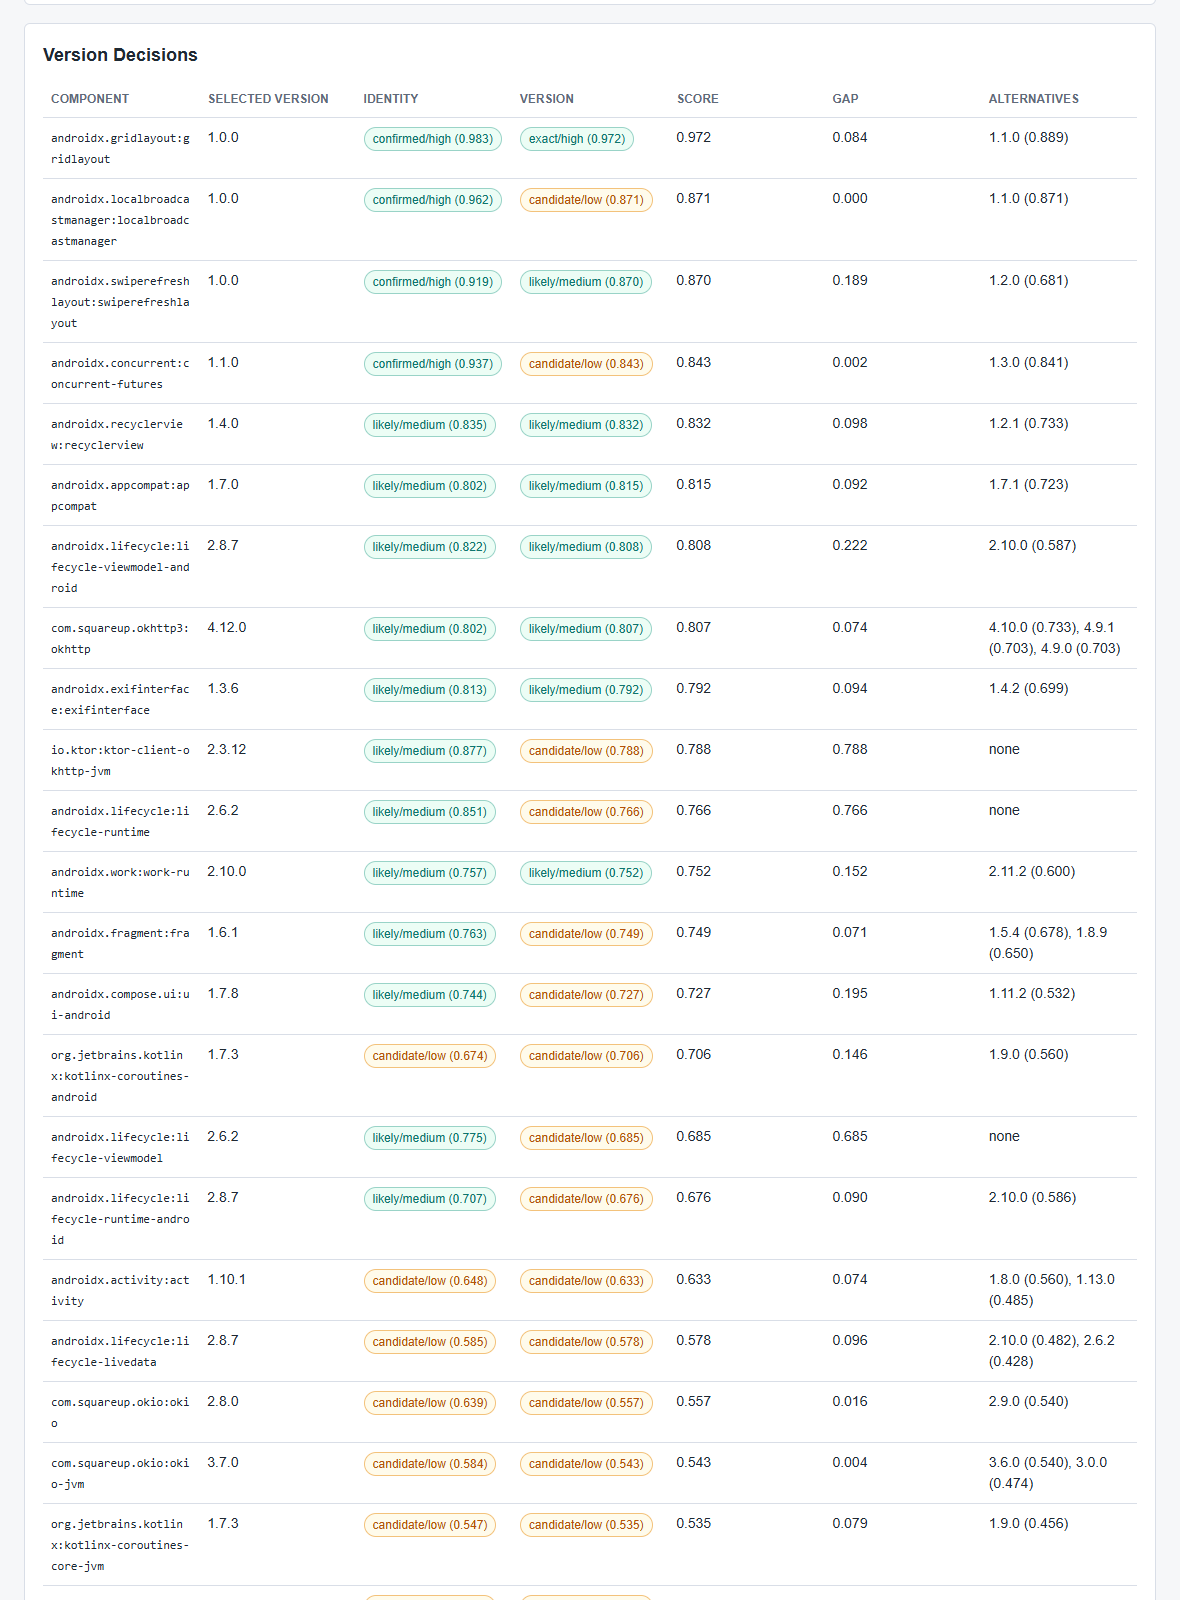
\includegraphics[width=\textwidth,height=0.78\textheight,keepaspectratio]{figures/clean-dashboard-04-version-decisions-a.png}
\caption[Clean dashboard: version decisions I]{Clean F-Droid dashboard,
version-decision panel, part I. The table exposes selected versions,
identity/version confidence, scores, score gaps, and alternatives for
analyst review.}
\label{fig:pfe-dashboard-clean-decisions-a}
\end{figure}

\begin{figure}[p]
\centering
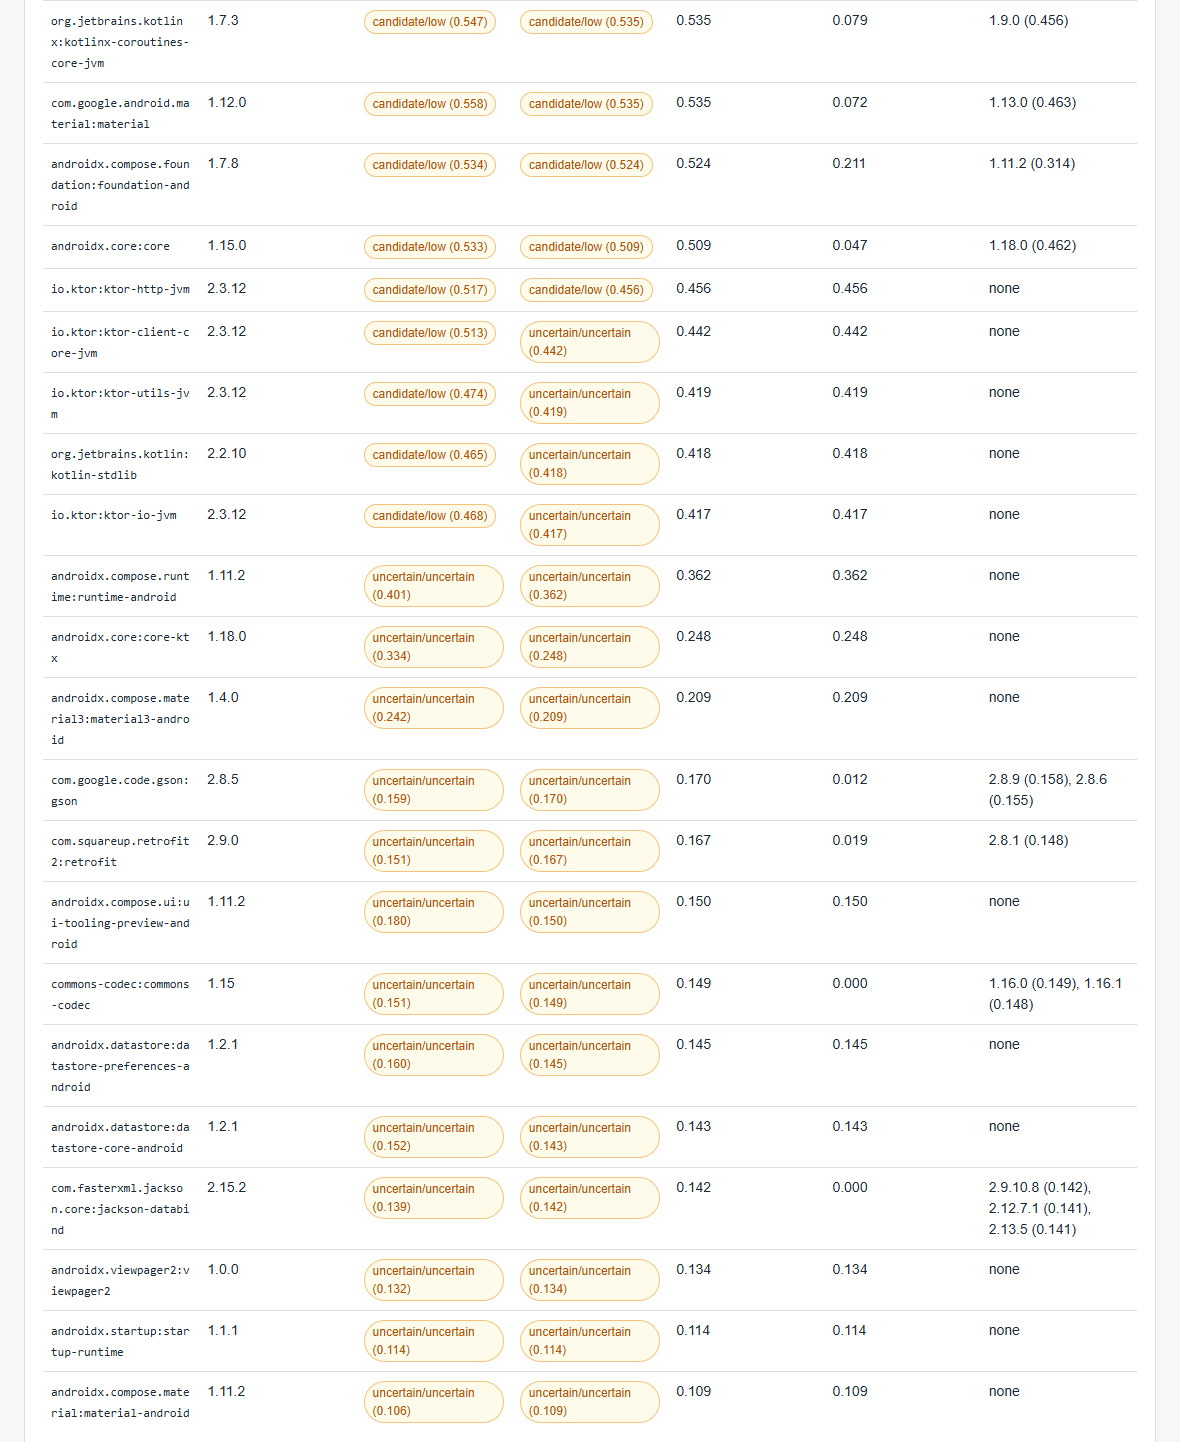
\includegraphics[width=\textwidth,height=0.78\textheight,keepaspectratio]{figures/clean-dashboard-05-version-decisions-b.png}
\caption[Clean dashboard: version decisions II]{Clean F-Droid dashboard,
version-decision panel, part II. Low-scoring and near-tied rows remain visibly
uncertain, which is essential to the confidence-aware reporting policy.}
\label{fig:pfe-dashboard-clean-decisions-b}
\end{figure}

\begin{figure}[p]
\centering
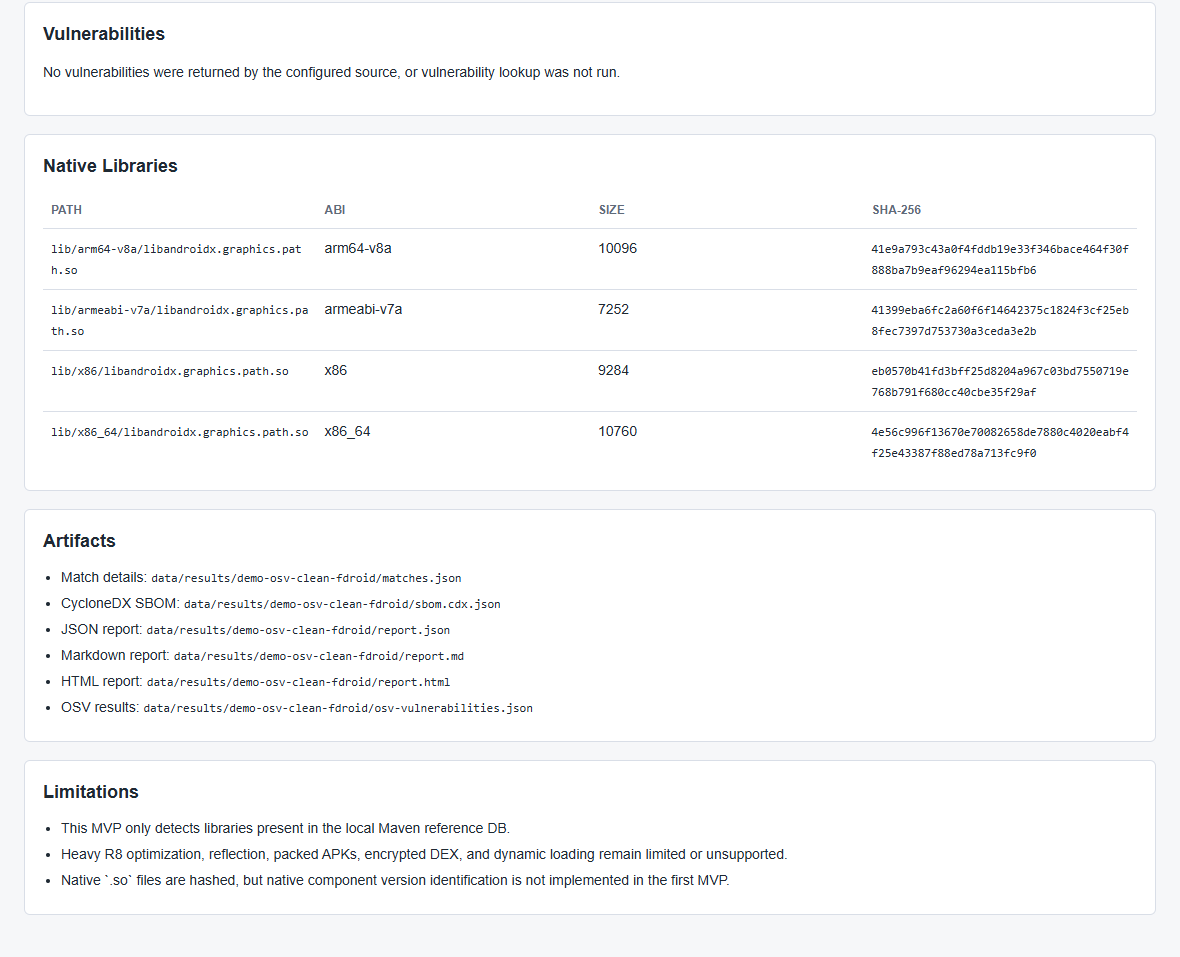
\includegraphics[width=\textwidth,height=0.78\textheight,keepaspectratio]{figures/clean-dashboard-06-vulnerabilities-artifacts.png}
\caption[Clean dashboard: findings and artifacts]{End of the complete clean
F-Droid dashboard: no returned vulnerabilities, four hashed native-library
artifacts, persisted JSON/Markdown/HTML/CycloneDX/OSV outputs, and explicit
MVP limitations.}
\label{fig:pfe-dashboard-clean-tail}
\end{figure}

\begin{figure}[p]
\centering
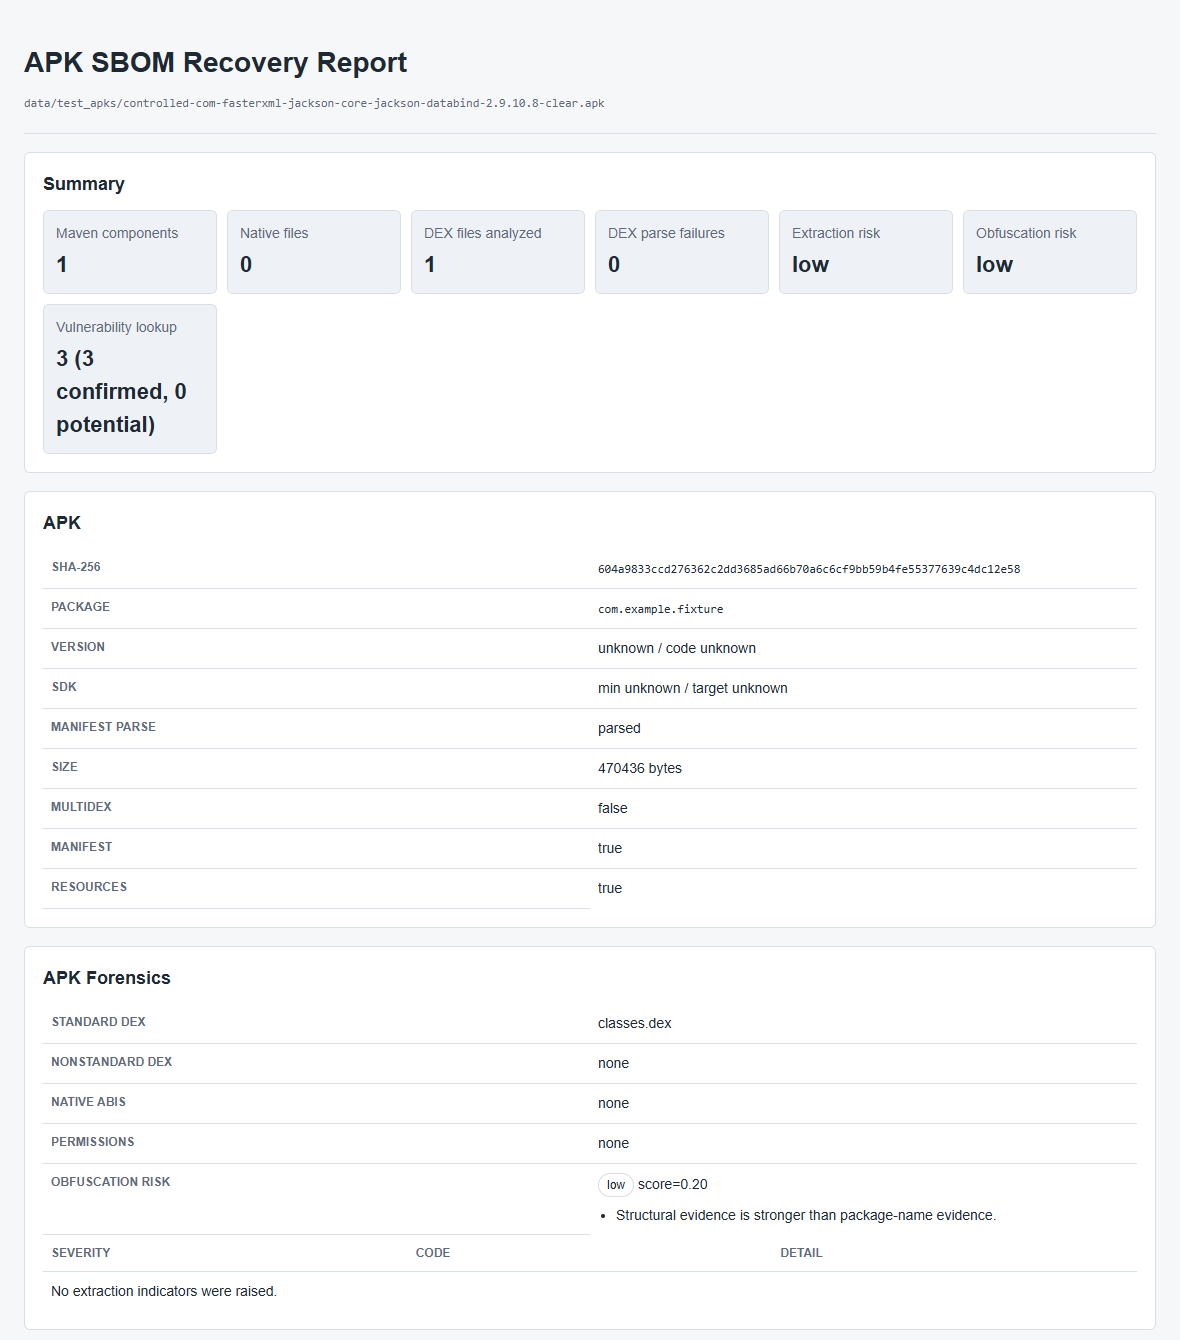
\includegraphics[width=\textwidth,height=0.78\textheight,keepaspectratio]{figures/vulnerable-dashboard-01-summary.png}
\caption[Vulnerable dashboard: summary and APK evidence]{Beginning of the
complete controlled vulnerable Jackson dashboard: one detected Maven
component, exact report processing, and three confirmed vulnerability
findings.}
\label{fig:pfe-dashboard-vulnerable-summary}
\end{figure}

\begin{figure}[p]
\centering
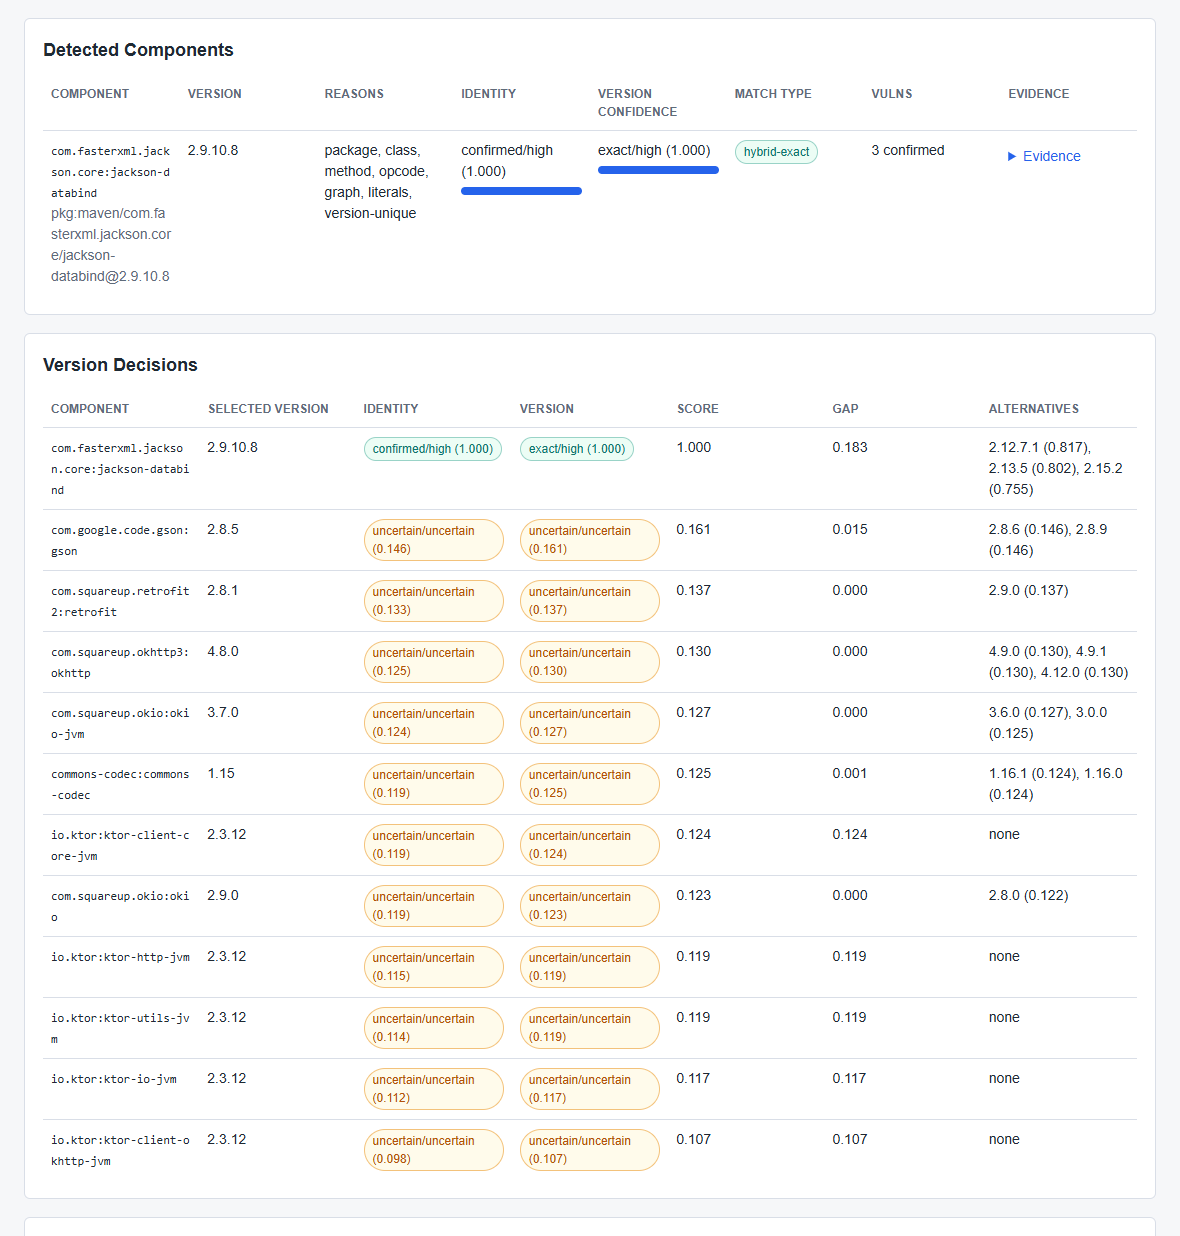
\includegraphics[width=\textwidth,height=0.78\textheight,keepaspectratio]{figures/vulnerable-dashboard-02-components-decisions.png}
\caption[Vulnerable dashboard: component and version evidence]{Controlled
vulnerable dashboard component and version-decision panels. Jackson Databind
2.9.10.8 receives exact/high identity and version confidence, while unrelated
low-scoring alternatives remain uncertain and are not emitted as components.}
\label{fig:pfe-dashboard-vulnerable-decisions}
\end{figure}

\begin{figure}[p]
\centering
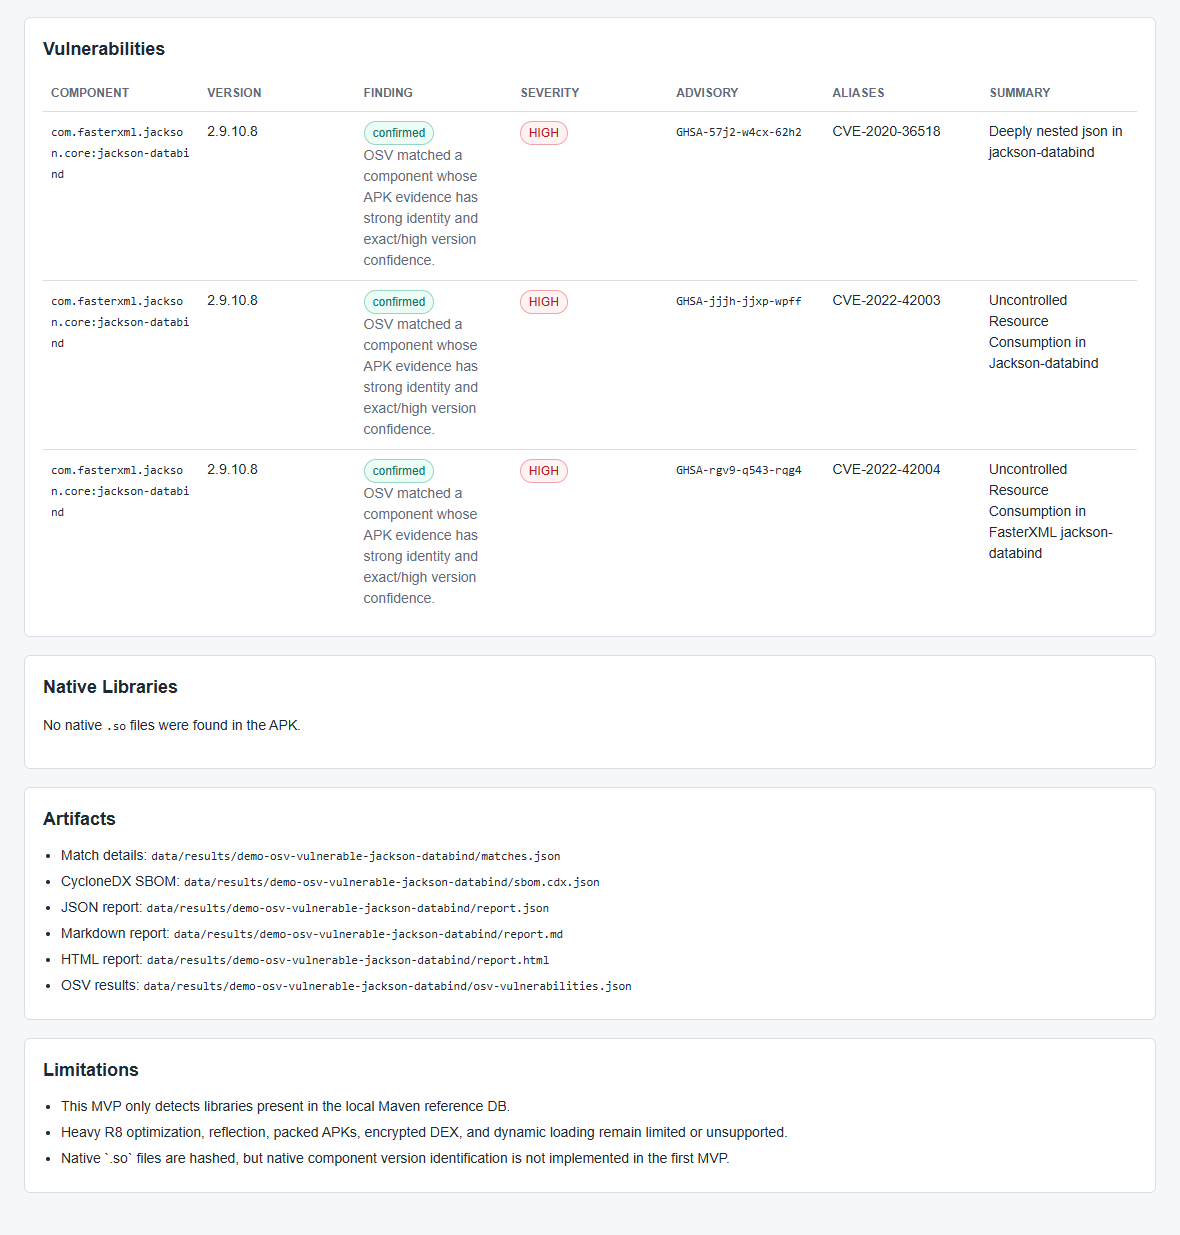
\includegraphics[width=\textwidth,height=0.78\textheight,keepaspectratio]{figures/vulnerable-dashboard-03-cves-artifacts.png}
\caption[Vulnerable dashboard: CVEs and artifacts]{End of the complete
controlled vulnerable dashboard: OSV maps Jackson Databind 2.9.10.8 to three
confirmed HIGH findings, CVE-2020-36518, CVE-2022-42003, and CVE-2022-42004,
then lists all persisted artifacts and the implementation limitations.}
\label{fig:pfe-dashboard-vulnerable-tail}
\end{figure}

\FloatBarrier

The result demonstrates why vulnerability scanning cannot be separated from
component attribution. OSV may correctly report advisories for the selected
version while the selected version itself disagrees with source evidence.
Applying source-validation labels therefore reduces false certainty without
discarding potentially useful triage information.

\section{AI and R8 Evaluation}

The AI layer was evaluated after the deterministic pipeline and evidence
exports were available. Its purpose is risk triage and investigation routing,
not direct component authority.

\begin{table}[H]
\centering
\caption{Machine-learning and Transformer results with authority decisions.}
\label{tab:pfe-ai-results}
\begin{tabularx}{\textwidth}{L{0.25\textwidth}L{0.22\textwidth}L{0.19\textwidth}X}
\toprule
\textbf{Model or gate} & \textbf{Dataset} & \textbf{Result} &
\textbf{Decision}\\
\midrule
Random Forest assistant & 20,523 project evidence rows, grouped by case &
Macro-F1 0.708; accuracy 0.690 & Integrated as report-only assistance.\\
Structured-token Transformer & 20,523 rows & Macro-F1 0.977 &
Research-status result; shortcut/context risk prevents authority.\\
MVP-safe Transformer & 20,523 rows with source/version shortcuts removed &
Macro-F1 0.882; accuracy 0.907 & Candidate for report-only risk triage;
production decision wiring disabled.\\
Raw-opcode Transformer & 1,680 method sequences from 14 APKs & Macro-F1 0.110
versus opcode-count baseline 0.128 & Negative result; research-only and not
promotable.\\
Strict APK-only promotion matrix & Five guarded profiles & 0 eligible
production candidates after controls & Matcher, SBOM, and CVE authority
remain blocked.\\
\bottomrule
\end{tabularx}
\end{table}

\subsection{AI Evidence Dataset}

The AI dataset is derived from project evidence produced by the matcher,
source-validation workflow, R8 diagnostics, and report-generation pipeline. It
is not an external Android machine-learning benchmark. The purpose of the
dataset is to train assistants that classify evidence rows into report actions
while preserving the deterministic matcher as the only SBOM authority. The
20,523 training-eligible rows cover 149 case identifiers and 1,370 Maven
coordinates. They are split by case identifier rather than by individual row:
14,905 rows from 104 cases are used for training, 1,750 rows from 15 cases are
used for validation, and 3,868 rows from 30 cases are used for testing. This
grouped split reduces direct leakage between near-duplicate rows from the same
APK or experiment.

\begin{table}[H]
\centering
\caption{AI evidence dataset composition.}
\label{tab:pfe-ai-dataset-composition}
\begin{tabularx}{\textwidth}{L{0.28\textwidth}rX}
\toprule
\textbf{Evidence source} & \textbf{Rows} & \textbf{Role in the AI task}\\
\midrule
Boundary evidence & 11,184 & Rows that encode authority boundaries,
limitations, and unsupported claims.\\
Emitted result & 6,772 & Source-known emitted rows used to learn
confirmed and reportable evidence states.\\
Matcher recall & 2,281 & Candidate rows that expose missing-reference and
retrieval limitations.\\
Phase 5 diagnostics & 286 & R8 and diagnostic rows used to connect
obfuscation evidence with report-only recommendations.\\
\bottomrule
\end{tabularx}
\end{table}

The label space is intentionally operational. Labels do not claim universal
APK ground truth; they describe how an analyst-facing report should treat a
row given the project evidence available for that row. The largest class,
\texttt{risk\_only}, contains 7,811 rows, while the smallest class,
\texttt{mismatch\_or\_extra}, contains 594 rows. This imbalance motivates
balanced class weights for the Random Forest and macro-averaged metrics for
all multi-class models.

\begin{table}[H]
\centering
\caption{AI training labels and their report meaning.}
\label{tab:pfe-ai-label-distribution}
\begin{tabularx}{\textwidth}{L{0.28\textwidth}rX}
\toprule
\textbf{Label} & \textbf{Rows} & \textbf{Meaning}\\
\midrule
\texttt{risk\_only} & 7,811 & Preserve the row as risk or analyst attention,
without claiming component authority.\\
\texttt{confirmed\_exact} & 6,790 & The evidence is consistent with an exact
source-confirmed row.\\
\texttt{boundary\_do\_not\_suggest} & 3,029 & The row falls under a boundary
condition and should not be promoted.\\
\texttt{suggest\_report\_only} & 1,429 & The row may be useful as a
report-only investigation suggestion.\\
\texttt{suppress\_uncertain} & 870 & Unsupported wording should be weakened or
removed from the analyst report.\\
\texttt{mismatch\_or\_extra} & 594 & The row conflicts with source evidence or
belongs to an extra unmatched candidate group.\\
\bottomrule
\end{tabularx}
\end{table}

\subsection{Random Forest Assistant}

The first report assistant is a \texttt{RandomForestClassifier}. It uses 200
trees, a maximum depth of 8, balanced class weights, random state 42, and 17
input features. The main feature families are identity and version confidence
scores, matcher scores, source rank, dependency/opcode scores, overlap
counts, and context flags. The resulting model reaches 0.7076 macro-F1 and
0.6903 accuracy on the grouped test split. The majority-class baseline reaches
0.3834 accuracy, and a simple score-threshold rule reaches 0.1655 accuracy.
These baselines are reported as accuracies because the generated baseline
artifacts did not compute macro-F1.

\begin{table}[H]
\centering
\caption{Random Forest configuration and baseline comparison.}
\label{tab:pfe-ai-rf-configuration}
\begin{tabularx}{\textwidth}{L{0.35\textwidth}X}
\toprule
\textbf{Item} & \textbf{Value}\\
\midrule
Model & \texttt{RandomForestClassifier}\\
Trees / depth & 200 trees; maximum depth 8\\
Class weighting & Balanced\\
Input features & 17 structured evidence features\\
Test result & Macro-F1 0.7076; accuracy 0.6903\\
Majority baseline & Accuracy 0.3834\\
Score-threshold baseline & Accuracy 0.1655\\
\bottomrule
\end{tabularx}
\end{table}

Feature importance shows that the model relies most heavily on confidence and
context features. The strongest features are \texttt{identity\_confidence}
(0.2307), \texttt{is\_boundary\_or\_limitation} (0.2170), \texttt{best\_score}
(0.2063), \texttt{source\_rank} (0.0855), \texttt{dependency\_score}
(0.0679), and \texttt{opcode\_score} (0.0489). These values explain how the
fitted forest used its inputs; they do not prove a causal relationship between
a feature and a correct security decision.

\begin{table}[H]
\centering
\caption{Random Forest ablation results.}
\label{tab:pfe-ai-rf-ablation}
\begin{tabularx}{\textwidth}{L{0.34\textwidth}r r X}
\toprule
\textbf{Variant} & \textbf{Features} & \textbf{Macro-F1} &
\textbf{Interpretation}\\
\midrule
All features & 17 & 0.7076 & Main report-only assistant.\\
No overlap counts & 14 & 0.7098 & Slightly higher, showing raw overlap counts
are not the main useful signal in this bounded task.\\
No context flags & 13 & 0.5639 & Large drop; context and boundary flags matter.\\
Scores only & 10 & 0.5579 & Scores alone are insufficient for the full
triage label space.\\
Overlap counts only & 3 & 0.1764 & Weak isolated signal.\\
Context flags only & 4 & 0.1619 & Weak isolated signal despite being useful
with other features.\\
\bottomrule
\end{tabularx}
\end{table}

The weakest Random Forest classes are the adjacent risk and mismatch labels.
For \texttt{risk\_only}, precision is 0.9906, recall is 0.2138, and F1 is
0.3516. For \texttt{mismatch\_or\_extra}, precision is 0.1010, recall is
0.7820, and F1 is 0.1788. Among 1,483 true \texttt{risk\_only} test rows, 926
are predicted as \texttt{mismatch\_or\_extra} and 222 as
\texttt{boundary\_do\_not\_suggest}. This weakness is acceptable only because
the model is used to guide report review. It would be unacceptable for
component, version, or vulnerability authority.

\subsection{Structured-Token Transformer}

The second assistant uses a \texttt{torch.nn.TransformerEncoder} with
64-dimensional embeddings, four attention heads, one encoder layer, sequence
length 64, batch size 128, and random state 42. The full token profile uses
20,523 rows and a 5,097-token vocabulary. It reaches 0.9478 validation
macro-F1, 0.9772 test macro-F1, and 0.9920 test accuracy. This result is
strong, but the full profile includes raw coordinate tokens, source-version
tokens, raw candidate-version tokens, structured features, and diagnostic
context labels. These inputs may encode shortcuts connected to how the project
labels were generated, so the result is retained as research workflow
evidence rather than deployment performance.

The MVP-safe profile removes source-version tokens, raw candidate-version
tokens, raw coordinate tokens, \texttt{source\_rank}, boundary/clean/partial
role flags, and diagnostic context labels. It retains source-free feature
buckets, tokenized group and artifact parts, candidate-version shape, and the
R8/minification flag. This profile uses a 1,704-token vocabulary and reaches
0.8600 validation macro-F1, 0.8822 test macro-F1, and 0.9069 test accuracy.
The reduction from 0.9772 to 0.8822 macro-F1 is important: it shows that the
safer profile is less shortcut-driven, but it still remains project-derived
and report-only.

\begin{table}[H]
\centering
\caption{Structured-token Transformer profiles.}
\label{tab:pfe-ai-transformer-profiles}
\begin{tabularx}{\textwidth}{L{0.22\textwidth}L{0.25\textwidth}X}
\toprule
\textbf{Profile} & \textbf{Metrics} & \textbf{Authority decision}\\
\midrule
Full profile & Vocabulary 5,097; validation macro-F1 0.9478; test macro-F1
0.9772; test accuracy 0.9920 & Research-status result because source and
context shortcuts may be present.\\
MVP-safe profile & Vocabulary 1,704; validation macro-F1 0.8600; test
macro-F1 0.8822; test accuracy 0.9069 & Candidate for report-only triage;
production decision wiring remains disabled.\\
\bottomrule
\end{tabularx}
\end{table}

\subsection{Raw-Opcode Transformer}

The raw-opcode experiment tests whether method-level opcode sequences alone
can support a learned diagnostic lane. The corpus contains 14 APKs, 1,680
method opcode sequences, seven labels, a 135-token vocabulary, and a maximum
sequence length of 128. For each label, one APK case is held out for test.
Validation rows are selected deterministically from the remaining training
cases because only two APK cases are available per label. The labels describe
R8 and real-APK profiles; they do not describe library coordinates or exact
versions.

\begin{table}[H]
\centering
\caption{Raw-opcode Transformer comparison.}
\label{tab:pfe-ai-raw-opcode-results}
\begin{tabularx}{\textwidth}{L{0.38\textwidth}r r X}
\toprule
\textbf{Model} & \textbf{Macro-F1} & \textbf{Accuracy} &
\textbf{Decision}\\
\midrule
Majority class & 0.0357 & 0.1429 & Minimal baseline.\\
Opcode-count logistic regression & 0.1281 & 0.1464 & Best simple baseline.\\
Raw-opcode Transformer & 0.1098 & 0.1464 & Below the logistic-regression
baseline; retained as negative evidence.\\
\bottomrule
\end{tabularx}
\end{table}

The raw-opcode Transformer does not justify promotion. Its macro-F1 is 0.0183
below the opcode-count logistic-regression baseline. The permitted conclusion
is therefore narrow: raw method-level opcode sequences alone did not improve
the assistant on this small case-heldout corpus. Future work needs more APK
cases, richer class/package context, and APK-level aggregation before raw
opcode learning can be reconsidered.

\subsection{Report-Only Integration Gate}

The integration gate verifies that AI can be displayed without changing
authoritative outputs. A two-target smoke test compares default reports with
opt-in hybrid/AI reports for F-Droid and Aegis Authenticator. Hybrid sections
are visible, but detected components, selected versions, CycloneDX component
content, vulnerability output, and the default matcher all remain unchanged.
The opt-in flag is \texttt{--include-hybrid-ai-assistance}. The generated
gate therefore permits report wording, risk and investigation triage, strategy
routing, model status, and metric reporting. It forbids automatic selected
version changes, automatic CycloneDX component or version changes, automatic
CVE/OSV label changes, source-validation metric changes, and raw-opcode
Transformer decision authority. The resulting integration level is
\texttt{production-report-only-ai-assistance}; matcher authority and SBOM/CVE
authority remain false.

A report-only smoke test confirms the authority boundary: enabling AI sections
leaves detected components, selected versions, semantically normalized SBOM
content, and vulnerability labels unchanged.

Figures~\ref{fig:pfe-dashboard-r8-diagnostics}
to~\ref{fig:pfe-dashboard-dl-results} show the corresponding report surface on
the hard Aegis real-APK lane. The screenshots are implementation evidence for
the R8/ML/DL layer, not additional accuracy measurements. Every panel states
or preserves the report-only boundary, and the deterministic weighted matcher
remains the SBOM authority.

\begin{figure}[p]
\centering
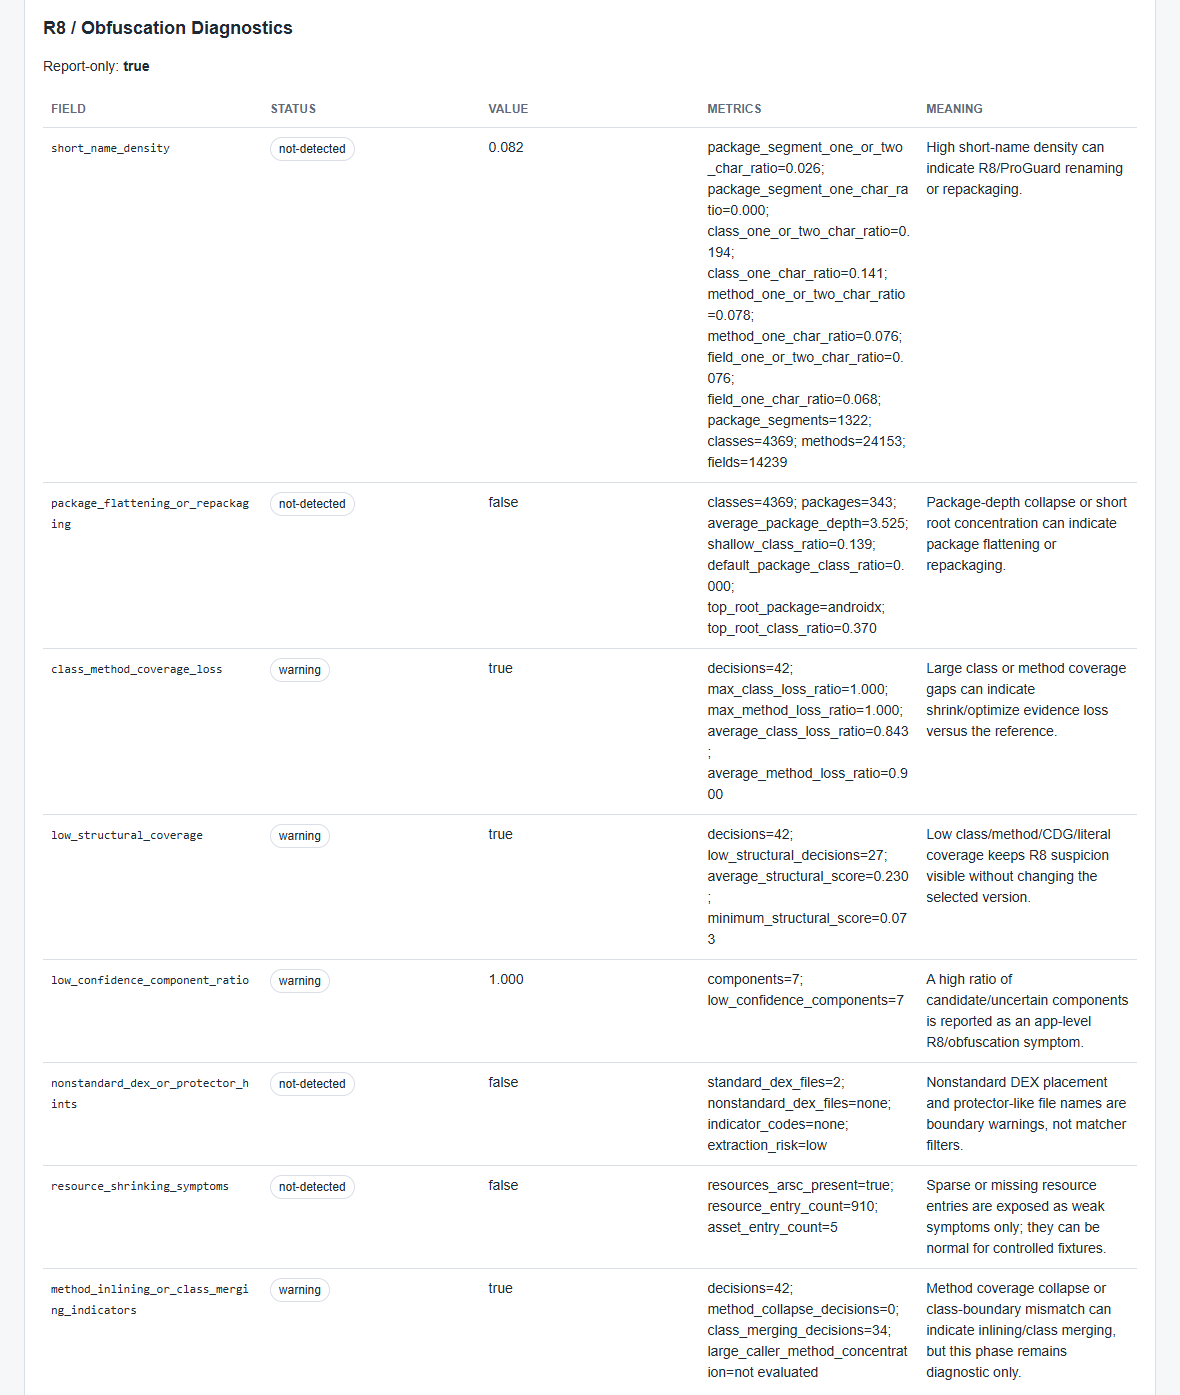
\includegraphics[width=\textwidth,height=0.78\textheight,keepaspectratio]{figures/hybrid-dashboard-01-r8-diagnostics.png}
\caption[R8 dashboard: report-only diagnostics]{Rendered R8/obfuscation
diagnostics from the Aegis hybrid report. Short-name density, package
flattening, coverage loss, structural coverage, low-confidence ratios,
protector hints, resource shrinking, and inlining/class-merging indicators are
reported without changing matcher scores or selected versions.}
\label{fig:pfe-dashboard-r8-diagnostics}
\end{figure}

\begin{figure}[p]
\centering
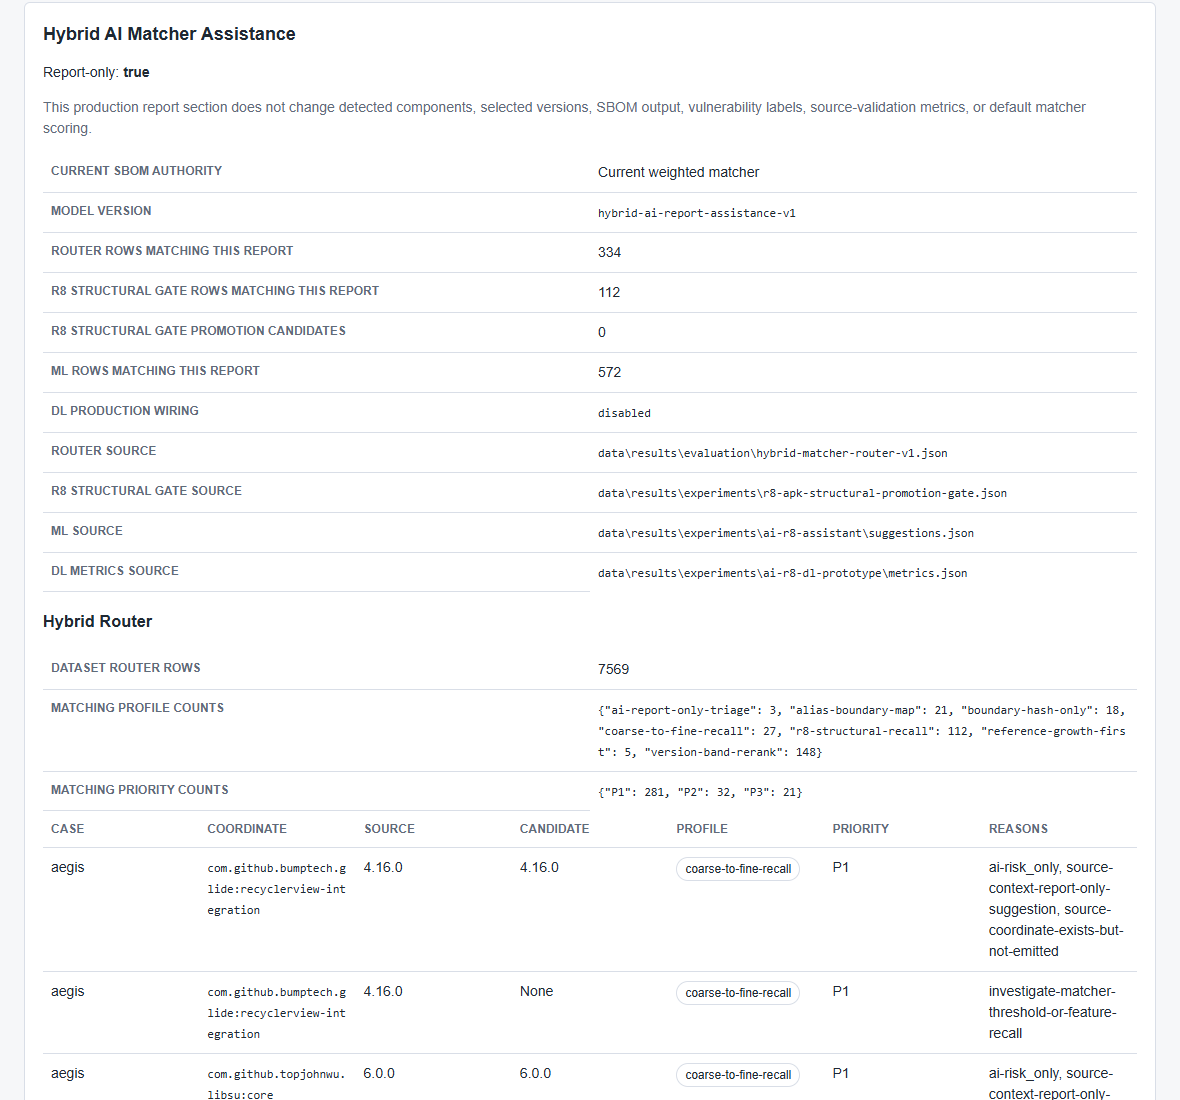
\includegraphics[width=\textwidth,height=0.78\textheight,keepaspectratio]{figures/hybrid-dashboard-02-assistance-summary.png}
\caption[Hybrid dashboard: authority and integration summary]{Hybrid AI
assistance summary for Aegis. The dashboard explicitly identifies the current
weighted matcher as the SBOM authority, marks the section report-only, reports
334 router rows, 112 R8 structural-gate rows, zero promotion candidates, 572
matching ML rows, and disabled DL production wiring.}
\label{fig:pfe-dashboard-hybrid-summary}
\end{figure}

\begin{figure}[p]
\centering
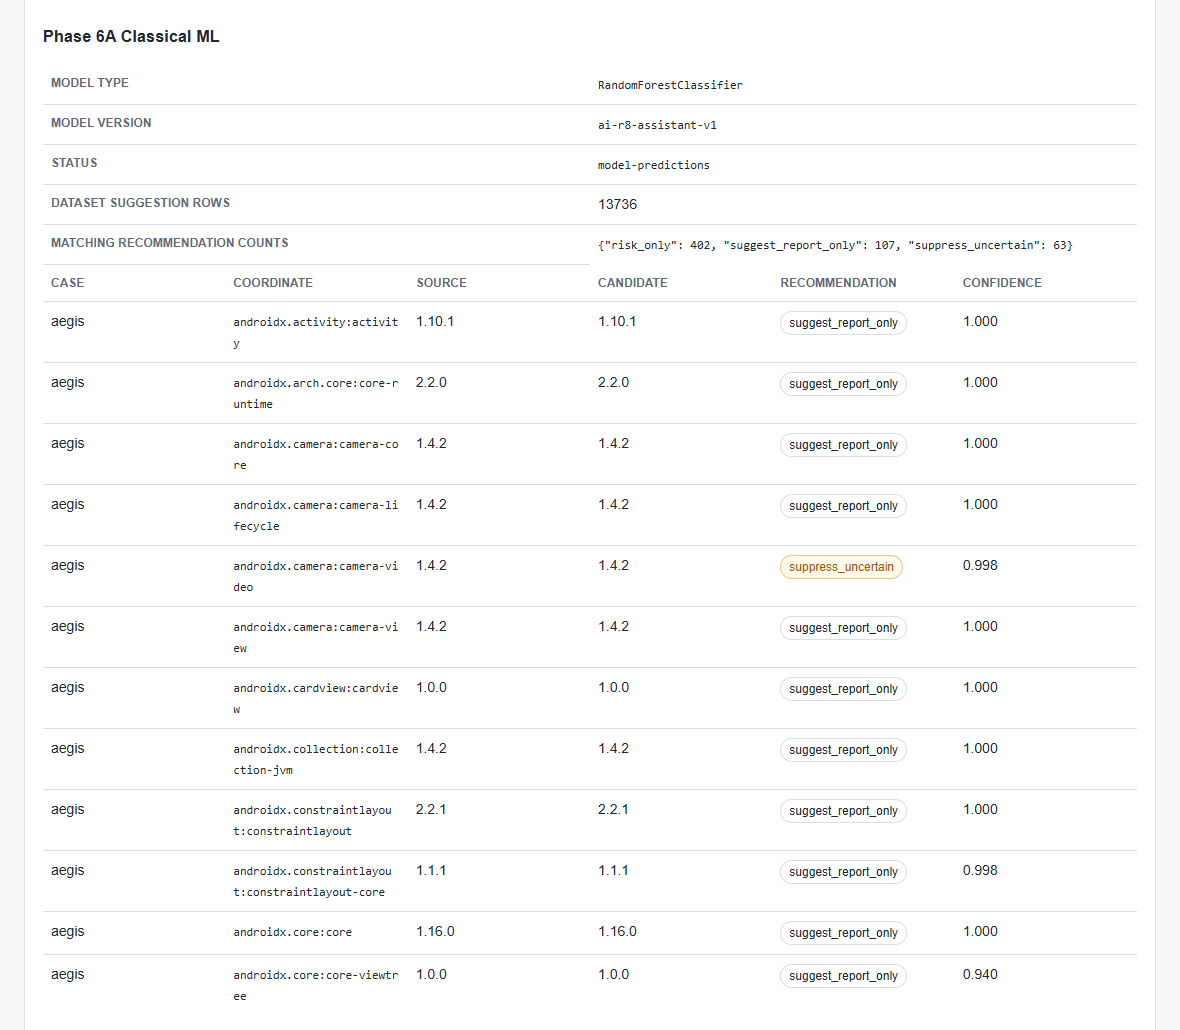
\includegraphics[width=\textwidth,height=0.78\textheight,keepaspectratio]{figures/hybrid-dashboard-03-ml-results.png}
\caption[ML dashboard: report-only recommendations]{Phase 6A Random Forest
report output for Aegis. The panel exposes the trained model, 13,736 dataset
suggestion rows, report-only recommendation counts, per-coordinate
recommendations, and confidence values for analyst triage.}
\label{fig:pfe-dashboard-ml-results}
\end{figure}

\begin{figure}[p]
\centering
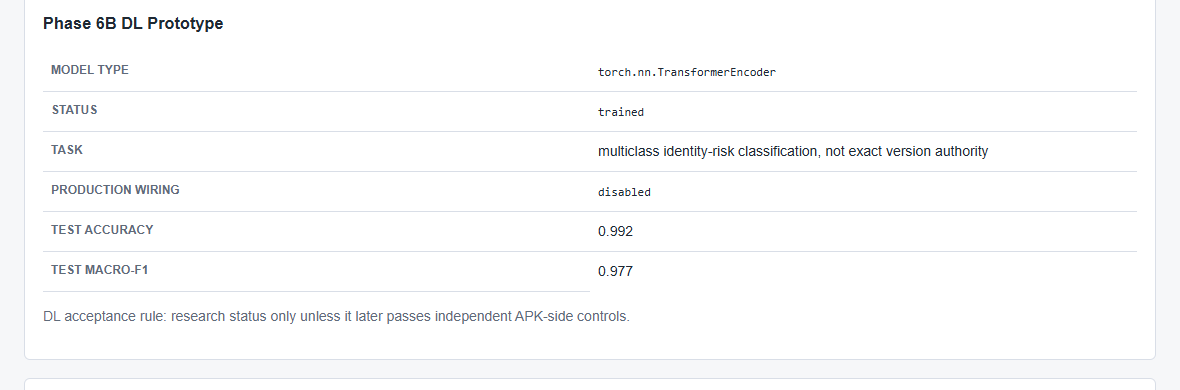
\includegraphics[width=\textwidth,height=0.78\textheight,keepaspectratio]{figures/hybrid-dashboard-04-dl-results.png}
\caption[DL dashboard: research-status result]{Phase 6B Transformer status in
the generated report. The model is trained and records test accuracy 0.992 and
macro-F1 0.977 for multiclass identity-risk classification, but production
wiring is disabled and exact-version authority remains explicitly excluded.}
\label{fig:pfe-dashboard-dl-results}
\end{figure}

\FloatBarrier

\section{Failed and Non-Promoted Experiments}

Negative experiments are part of the contribution because they show which
apparently promising changes were rejected by target/control evidence.

\begin{table}[H]
\centering
\caption{Representative failed, blocked, or non-promoted experiments.}
\label{tab:pfe-failed-experiments}
\begin{tabularx}{\textwidth}{L{0.23\textwidth}L{0.23\textwidth}X}
\toprule
\textbf{Experiment} & \textbf{Observed result} & \textbf{Decision and lesson}\\
\midrule
Global opcode tri-gram weight & Regressed established controls without a
confirmed-version gain & Disabled by default; a useful signal is not
automatically a safe global weight.\\
Global API-reference weight & Changed no guarded source-validation metric &
Disabled by default because no measured benefit justified extra authority.\\
Global multi-scale R8 blend & Found four target improvements but also six
controlled, 30 real source-validated, and eight clean-real regressions &
Rejected globally; retained as diagnostic features and narrower report-only
experiments.\\
Version-band reranking & 565 wrong-version rows appear fixable under
source-known constraints; APK-only safe fixes remained 0 & Not promoted;
source-known opportunity is not APK-only evidence.\\
Deep candidate expansion & Rescoring 134 Activity versions selected an older,
incorrect alpha release & Not promoted; a larger candidate set requires
stronger version-specific evidence.\\
Priority reference database & Exact source-version coverage reached 79.9\%,
but I2P output expanded from 18 rows to 111 in the broad preflight and
introduced 14 source-missing rows & Fail-fast rejection for production-style
use; database remains evaluation-only.\\
Fragment 1.6.2 & Ten affected rows selected 1.6.2 and sampled controls stayed
clean, but 1.6.1/1.6.2 retained very small candidate-level score gaps without
matched version-unique APK evidence &
Experiment-only; no shared DB promotion without version-unique APK evidence.\\
Raw-opcode Transformer & Macro-F1 0.110, below baseline 0.128 & Honest
negative result; larger and richer bytecode context is required.\\
\bottomrule
\end{tabularx}
\end{table}

These outcomes support the fail-fast policy. The project favors a stable,
bounded default over a larger but poorly controlled result surface.

\section{Comparison with Existing Work}

Chapter~\ref{ch:pfe-sota} reviews Android library detectors whose objectives,
datasets, and metrics differ substantially. Consequently, this thesis does
not rank the MVP against reported percentages from incompatible benchmarks.
Instead, Table~\ref{tab:pfe-dimensional-comparison} compares capabilities that
can be stated consistently.

\begin{table}[H]
\centering
\caption{Dimension-based positioning relative to the reviewed detector
families.}
\label{tab:pfe-dimensional-comparison}
\begin{tabularx}{\textwidth}{L{0.25\textwidth}L{0.31\textwidth}X}
\toprule
\textbf{Dimension} & \textbf{Common emphasis in prior work} &
\textbf{Implemented MVP position}\\
\midrule
Primary objective & Library presence, similarity, or version detection &
End-to-end evidence recovery, SBOM emission, validation, and vulnerability
interpretation.\\
Reference representation & Class, package, hash, opcode, API, graph, or
learned profiles & Hybrid DEX profile with name, opcode, literal, API,
dependency, and guarded contextual signals.\\
Version uncertainty & Often one top candidate or threshold decision &
Separate identity/version confidence, alternatives, and ambiguous version
sets.\\
Obfuscation handling & Technique-specific robustness evaluations &
Controlled R8 categories, real minified cases, and explicit report-only
diagnostics.\\
Standard SBOM output & Frequently absent from detector prototypes &
\CycloneDX 1.5 with PURLs, evidence properties, and native file hashes.\\
Vulnerability mapping & Often a downstream security use case &
OSV integration with source-aware confirmed, potential, and report-only
labels.\\
Negative experiments & Usually secondary to the promoted method &
Preserved in a decision ledger and used to block unsafe promotion.\\
Full denominator transparency & Often benchmark-specific &
Emitted-version quality, full source dependency coverage, and source-known
upper bound reported separately.\\
\bottomrule
\end{tabularx}
\end{table}

The main engineering difference is therefore integration and evidence
governance, not a claim that one similarity function universally outperforms
all prior detectors.

\section{Discussion}

\subsection{Answers to the Research Questions}

\textbf{RQ1: Can exact versions be recovered?} Yes, under bounded conditions.
The system confirms 84/84 controlled expected versions and 47/47 emitted
versions in the clean real slice. The partial and full-denominator results
show that this capability does not generalize uniformly across all source
dependencies.

\textbf{RQ2: How does behavior change across APK families?} Clean,
well-covered APKs support exact emission. Modern AndroidX/Kotlin, older
dependency eras, R8/minified, native-heavy, and large-tree applications
produce more adjacent-version mismatches and missing/nuanced rows. The
clean/partial split is therefore an essential result, not merely a reporting
choice.

\textbf{RQ3: What limits full recovery?} Both reference coverage and matcher
recall. The shared database covers the exact source version for 10.2\% of the
12,082 source rows, while end-to-end exact recall is 7.7\%. In the larger
source-known lane, the remaining actionable gaps divide into missing-reference
and matcher-recall candidates.

\textbf{RQ4: Can downstream output preserve uncertainty?} Yes. The SBOM stores
confidence and ambiguity properties, vulnerability findings can be relabeled
by source validation, native files remain hash-backed file components, and AI
assistance is report-only.

\subsection{Strengths}

The system's principal strengths are:

\begin{itemize}
  \item an operational path from compiled APK to standard SBOM and
  vulnerability report;
  \item a common DEX representation for APK and reference artifacts;
  \item separate library-identity and exact-version decisions;
  \item source-backed validation and a visible full dependency denominator;
  \item fail-fast target/control promotion rules;
  \item explicit native, hidden-code, and AI authority boundaries;
  \item reproducible machine-readable evidence and human-readable reports.
\end{itemize}

\subsection{Error Categories}

The current errors are not one homogeneous matcher failure. They include:

\begin{itemize}
  \item adjacent versions with nearly equivalent compiled evidence;
  \item public, Android-target, JVM, KTX, and sibling artifact families;
  \item source versions absent from the shared reference database;
  \item exact profiles present but not surfaced by candidate generation;
  \item metadata-only or platform dependencies that do not provide ordinary
  DEX bytecode;
  \item dependencies removed or transformed during building and shrinking;
  \item false-positive extra emissions encouraged by broad package overlap;
  \item native, dynamic, hidden, or protected code outside the current JVM
  attribution model.
\end{itemize}

\subsection{Practical Value of Partial Results}

A partial SBOM can still identify high-confidence components, document native
files, provide hashes, reveal version ambiguity, and guide vulnerability
investigation. Its practical value depends on preserving uncertainty. A
smaller evidence-qualified SBOM is safer than a larger list of precise-looking
but unsupported coordinates and versions.

\subsection{Runtime and Scalability}

SQLite lookup and APK DEX analysis are practical for focused and calibrated
databases. Broad evaluation databases introduce a different problem:
candidate generation must remain precise enough to avoid both excessive
runtime and false emissions. The priority-database preflight demonstrated that
package-overlap shortlists can recover intended rows while severely inflating
the output. A safer large-database deployment therefore requires a stronger
APK-only shortlist or candidate-emission gate rather than only additional
hardware or a larger database.

\section{Threats to Validity}

\subsection{Internal Validity}

Implementation defects, stale generated tables, or inconsistent configuration
could affect the results. These risks are reduced through automated tests,
generated thesis tables, explicit artifact paths, and a frozen evidence
snapshot. However, not every long-running APK evaluation is rerun for each
writing session.

\subsection{Construct Validity}

The emitted Maven version confirmation rate measures correctness among emitted
rows, not complete dependency recovery. Presenting it as full recall would be
a construct error. This chapter therefore reports the 12,082-row source
denominator separately.

Source dependency trees are strong external evidence, but they represent
resolved build dependencies rather than a perfect bytecode manifest. Gradle
may include BOMs, metadata, compile-time modules, transformed artifacts, and
dependencies removed by shrinking.

\subsection{External Validity}

The source-tree dataset contains 106 source-validated APKs with diverse
categories: 102 emit Maven rows and four are no-Maven-signal controls. It is
not a random sample of all Android applications. Open-source F-Droid and
GitHub projects are overrepresented because their source and dependency
evidence can be audited. Commercial protectors, games, Flutter, Unity, and
additional dynamically loaded applications require broader future datasets.

\subsection{Reference-Database Bias}

The selected reference database directly constrains what can be recognized.
A missing version can force a nearby candidate, while a broad database can
increase both runtime and false-positive pressure. The source-known v2 lane
measures a useful upper bound but cannot estimate unconstrained production
accuracy.

\subsection{AI Validity}

The AI datasets are derived from project evidence and are not an independent
external benchmark. The high full structured-token Transformer result may
benefit from contextual shortcuts. Grouped splits and the MVP-safe profile
reduce this risk, while the negative raw-opcode result demonstrates that a
more direct representation is not yet competitive. AI conclusions are
therefore limited to report-only assistance.

\section{Conclusion}

The implemented MVP provides a complete static APK-to-SBOM workflow:
extraction, DEX analysis, Maven reference matching, confidence-aware version
decisions, \CycloneDX generation, OSV lookup, source validation, and
multi-format reporting.

The evaluation establishes three bounded conclusions. First, the mechanics are
reliable on the controlled inventory and on the clean real emitted rows.
Second, difficult real APKs remain useful but expose substantial version and
coverage limitations: 927 of 1,837 emitted Maven versions are confirmed across
the 102 source-validated APKs that emit Maven rows, while four additional
source-validated cases remain no-Maven-signal controls. Exact end-to-end recall
against the full source denominator is 927 of 12,082. Third, the source-known
v2 and AI lanes are valuable diagnostic upper bounds and assistants, but their
authority remains separate from unconstrained APK-only SBOM decisions.

The final chapter synthesizes these contributions, limitations, and future
directions without converting experimental evidence into stronger claims than
the evaluation supports.
